\documentclass{ieeeaccess}
\usepackage{cite}
\usepackage{amsmath,amssymb,amsfonts}
\usepackage{graphicx}
\usepackage{xcolor}
\def\BibTeX{{\rm B\kern-.05em{\sc i\kern-.025em b}\kern-.08em}
    T\kern-.1667em\lower.7ex\hbox{E}\kern-.125emX}
\usepackage{stfloats}
\usepackage{url}
\usepackage{pifont}
\newcommand{\cmark}{\ding{51}}
\usepackage{booktabs}
\graphicspath{{figures/}}

% Allow standard figure environments with the IEEE Access caption formatter.
% Its custom \Figure command normally initializes this width.
\providecommand{\xfigwd}{\columnwidth}
% Replace this placeholder when the repository address is available.
\providecommand{\RepoURL}{\texttt{[repository URL pending]}}

% Visible working-draft queries. Resolve and remove every red query before
% submission, then switch \showopenissuesfalse for the clean manuscript.
\newif\ifshowopenissues
\showopenissuestrue
\newcommand{\openissue}[1]{%
  \ifshowopenissues\par\noindent
  {\color{red}\footnotesize\textbf{OPEN AUTHOR QUERY:} #1}\par\fi}

% Device-CMYK fallback for IEEE Access heading color in review PDFs.
\definecolor{accessblue}{cmyk}{1,0.3,0,0.2}
\definecolor{greycolor}{cmyk}{0,0,0,.8}

\begin{document}
\history{Date of publication xxxx 00, 0000, date of current version xxxx 00, 2026.}
\doi{XXXXXXXXX/ACCESS.2026.DOI}

\title{
From Reactive Vision-Language-Action Policies to Predictive World Models:
A Review for Robotic Manipulation}
\author{\uppercase{Muhayy Ud Din}\authorrefmark{1}, 
\uppercase{Ahsan B. Bakht}\authorrefmark{1}, 
\uppercase{Ibrar Yaqoob}\authorrefmark{2},
and \uppercase{Irfan Hussain}\authorrefmark{1}
}
\address[1]{Khalifa University Center for Autonomous Robotic Systems (KUCARS),
Khalifa University, Abu Dhabi 127788, United Arab Emirates.}
\address[2]{Artificial Intelligence and Cyber Futures Centre, Charles Sturt University, Bathurst, NSW, Australia.}

\tfootnote{This work is supported by the Khalifa University of Science and Technology under Awards Nos. 8434000534, CIRA-2021-085,
RC1-2018-KUCARS, KU-Stanford: 8474000605.\\
Corresponding author e-mail: irfan.hussain@ku.ac.ae}

%%%%%%%%%%%%%%%%%%%%%%%%%%%%%%%%%%%%%%%%%%%%%%%%%%%%%%%%%%%%%%%%%%%%%%%%%%%%%%%%

% =========================================================================
% ABSTRACT — <=250 words, no citations, acronyms defined at first use.
% =========================================================================
\begin{abstract}
\textcolor[RGB]{104,48,148}{Vision-language-action (VLA) policies connect visual observations and language instructions to robot actions, but benchmark success alone does not establish reliable behavior under physical interaction or distribution shift. This review examines the transition from direct action prediction toward predictive world models for robotic manipulation through a mapping of 144 reports. It organizes VLA systems and predictive mechanisms, distinguishes observed limitations from gaps in their evaluation, and assesses whether proposed mechanisms improve the relevant outcomes. Six limitation and evaluation-gap categories cover execution monitoring and recovery, distribution shift, data requirements, physical grounding, evaluation validity, and safety. Computational costs introduced by prediction and search are considered separately. Selected manipulation comparisons support synthetic-trajectory augmentation and auxiliary predictive training. Learned practice and candidate-action comparison show promise in narrower experiments, while physical validity, evaluation transfer, and calibrated safety remain incompletely established. Results are interpreted within their original tasks, baselines, and computational settings rather than combined into a cross-system ranking. The review concludes with a research agenda for control-oriented prediction, stable representations, data composition, functional evaluation, and dependable deployment. Verified imagination is framed as a proposed integration of learned dynamics with explicit planning constraints and runtime assurance, whose guarantees depend on stated assumptions about model error and operating conditions.}
\end{abstract}

\begin{IEEEkeywords}
Embodied artificial intelligence, model-based reinforcement learning, robot
learning, robotic manipulation, systematic mapping review, video prediction,
vision--language--action models, world models.
\end{IEEEkeywords}

\maketitle

\section{Introduction}
\label{sec:introduction}

\IEEEPARstart{R}{obotic} manipulation has advanced rapidly through vision-language-action (VLA) policies that translate visual observations and language instructions into robot actions. RT-2 established this paradigm by adapting a web-scale vision-language model to robotic data~\cite{rt2}. OpenVLA later provided an open implementation trained on the Open X-Embodiment corpus~\cite{openvla,oxe}. Recent systems such as $\pi_0$, GR00T~N1, Gemini Robotics, and Figure Helix have extended the approach to larger datasets and more diverse embodiments~\cite{pi0,groot,geminirobotics,gemini15}. \textcolor[RGB]{104,48,148}{Several VLA systems report success rates above 97\% under specified LIBERO configurations~\cite{openvlaoft,simplevlarl,cosmospolicy}.} These results demonstrate substantial progress under the evaluated protocols. However, they do not establish whether the same policies can remain reliable when the environment or task differs from the training distribution.

World models offer a complementary approach. A world model learns how an environment changes over time and how those changes depend on an agent's actions. It can support future-state prediction, imagined training, or planning before physical execution. These capabilities distinguish explicit predictive reasoning from a predominantly reactive policy interface. In this review, \emph{reactive} describes a policy that selects actions without exposing an action-conditioned transition model for comparing their predicted consequences. This definition does not imply that the policy lacks memory or an internal representation of dynamics. Reactive control and explicit planning instead represent different points along a continuum of predictive capability. Fig.~\ref{fig:timeline} traces the development of VLA policies and world models, together with their recent convergence into world-action systems.

%================================================================

\begin{figure*}[!t]
\centering
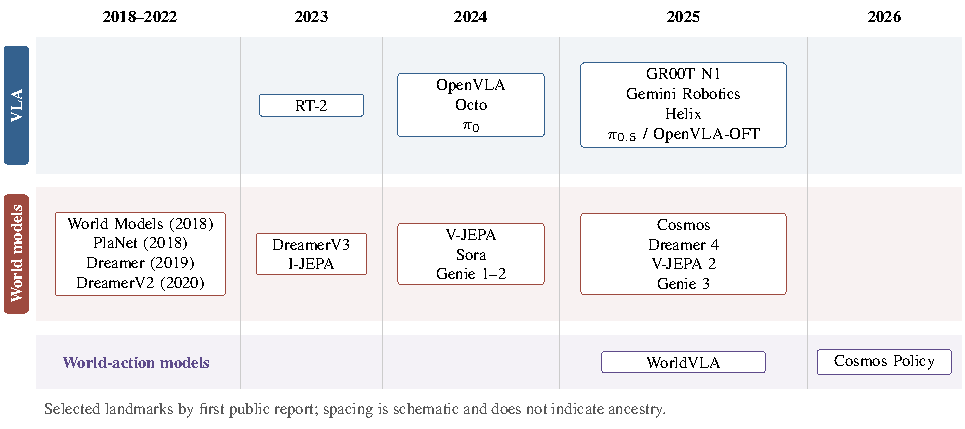
\includegraphics[width=0.95\linewidth]{figures/timeline.pdf}
\caption{\textcolor[RGB]{104,48,148}{Selected chronological landmarks in VLA policies, world models, and world-action models. Dates denote the first public paper or technical report, including preprints; later venue dates can differ. Horizontal spacing is schematic and does not imply architectural ancestry.}}
\label{fig:timeline}
\end{figure*}

%================================================================

The motivation for this convergence extends beyond benchmark performance. Perturbation studies show that VLA policies can degrade substantially under changes in layout, viewpoint, or instruction phrasing~\cite{liberoplus}. Real-to-simulation studies also question whether success on common benchmarks reliably predicts physical performance~\cite{polaris}. Reinforcement-learning post-training has produced large improvements over supervised policies in specific LIBERO settings~\cite{simplevlarl,riptvla}. However, these experiments change the training data and optimization process together, which makes the source of improvement difficult to isolate. Large teleoperation datasets further demonstrate the value of action-grounded experience while highlighting its acquisition cost~\cite{pi0}. Together, these findings expose a broader limitation: selecting actions from learned correlations is not the same as predicting their physical effects.

Predictive models could help address this limitation by allowing a robot to evaluate how alternative actions may change the environment. They could also provide imagined experience for policy learning. Yet prediction alone is not sufficient. A visually plausible future may violate contact dynamics or omit information that matters for control. Predictions may also become unreliable when actions fall outside the model's training support. A world model should therefore be treated as a candidate mechanism rather than a universal solution. Its value must be established through improvements in control and physical reliability, not through prediction quality alone.

Recent systems illustrate both the promise and the uncertainty of this direction. V-JEPA~2 combines large-scale video pretraining with action-conditioned adaptation for robotic manipulation~\cite{vjepa2}. DreamGen uses generated trajectories to expand the behavioral coverage of a robot policy~\cite{dreamgen}. Dreamer~4 demonstrates complex policy learning inside a learned environment, although its principal evidence comes from Minecraft rather than robotic manipulation~\cite{dreamer4}. WorldVLA jointly generates future video and robot actions~\cite{worldvla}, while Cosmos Policy adapts a video world model for direct control and rollout-based planning~\cite{cosmospolicy}. These developments indicate a movement toward unified world-action models. However, current evidence remains narrow and often combines several system components. It does not yet establish a general advantage for predictive planning in manipulation.

This review examines the transition from VLA policies to predictive systems through a systematic mapping of \textcolor[RGB]{104,48,148}{144 reports}. Rather than asking which architecture performs best, we focus on the relationship between limitations and proposed solutions. We first identify the major limitations affecting current VLA systems. We then examine which world-model mechanisms could address them. Finally, we assess whether the available evidence demonstrates the intended benefit. This structure separates evidence that a limitation exists from evidence that a mechanism changes it. It also distinguishes both from downstream task success.

Existing surveys provide broad accounts of VLA architectures and their deployment challenges~\cite{ma2024survey,zhong2025token,kawaharazuka2025,din2025priorvlasurvey}. A parallel literature reviews world models for robot learning and embodied artificial intelligence~\cite{hou2026wm,li2025wm,wang2026manipwmsurvey}. Recent studies also survey the emerging world-action-model paradigm~\cite{wamfrontier,wamsurvey}. The present article does not seek to reproduce these architectural taxonomies. Instead, it connects diagnosed VLA limitations to candidate predictive mechanisms and evaluates the strength of evidence supporting each connection. The scope is centered on robotic manipulation.

The article makes four principal contributions:

\begin{enumerate}
\item \textcolor[RGB]{104,48,148}{It organizes six limitations and evaluation gaps in current VLA research.} The analysis distinguishes limitations of policy formulation from those arising in training or evaluation.


\item It establishes a mechanism-centered connection between VLA policies and world models. The proposed limitation-to-candidate-mechanism framework separates direct evidence from indirect or prospective claims.

\item It provides a protocol-aware synthesis of empirical findings across both research areas. Benchmark results are interpreted within their original experimental settings rather than combined into a common leaderboard. \textcolor[RGB]{104,48,148}{The synthesis identifies evaluation and deployment considerations for comparing candidate model families.}

\item It presents a testable research agenda for dependable predictive manipulation. The agenda culminates in \emph{verified imagination}, which integrates learned dynamics with runtime monitoring and formal constraints. It also connects prediction with task-and-motion planning so that imagined outcomes can guide action without being treated as verified facts.


\end{enumerate}

The remainder of the article follows this argument. Section~\ref{sec:related} positions the review relative to existing surveys, and Section~\ref{sec:methodology} presents the mapping methodology. \textcolor[RGB]{104,48,148}{Sections~IV and V characterize VLA systems and their limitations. Section~VI maps these limitations to predictive mechanisms, while Section~VII examines benchmarks and interprets reported results.} Section~VIII develops the research agenda, and Section~IX concludes the article. Fig.~\ref{fig:paperroadmap} summarizes this progression.

%===========================

\begin{figure*}[!tb]
\centering
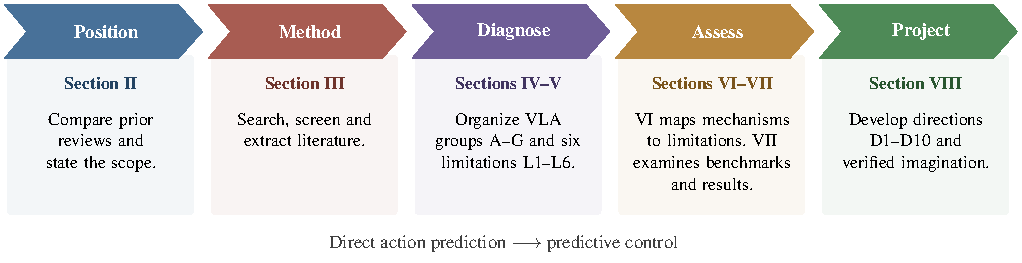
\includegraphics[width=0.99\linewidth]{figures/paper-roadmap.pdf}
\caption{\textcolor[RGB]{104,48,148}{Paper roadmap connecting survey positioning and review methodology with VLA analysis and limitation diagnosis, assessment of predictive mechanisms, and the research agenda.}}
\label{fig:paperroadmap}
\end{figure*}

% ==========================
\section{Related Surveys and Positioning}
\label{sec:related}

Surveys of VLA policies and world models have largely developed as separate literatures. VLA reviews typically focus on policy design and deployment, while world-model reviews emphasize predictive architectures and their roles in learning or planning. Table~\ref{tab:surveys} compares the studies most closely related to this review.

\subsection{Surveys of Vision-Language-Action Models}

The rapid growth of VLA research has produced surveys that examine the field from architectural, representational, and deployment perspectives. Ma \emph{et al.} organize VLA systems according to their components and control hierarchies~\cite{ma2024survey}. Zhong \emph{et al.} focus on action tokenization across discrete and continuous representations~\cite{zhong2025token}. Kawaharazuka \emph{et al.} examine real-world deployment, with particular attention to hardware integration and data collection~\cite{kawaharazuka2025}. Other reviews address general VLA concepts~\cite{sapkota2025}, large-VLM manipulation policies~\cite{shao2025}, efficient deployment~\cite{yu2025efficient}, and reinforcement-learning post-training~\cite{deng2025rl}.

\textcolor[RGB]{104,48,148}{Din \emph{et al.} review multimodal fusion in VLA models for robotic manipulation, covering 102 models together with datasets and simulation platforms~\cite{din2025priorvlasurvey}. Their focus is fusion strategy, architecture, and comparative performance. Section~IV of the present review supplies background on the same policy literature; this coverage is not claimed as a new VLA taxonomy. The contribution here is the joint analysis of VLA limitations, candidate predictive mechanisms, and the experiments that test their effects. World-model failure modes and the conditions needed for predictive planning extend the scope beyond the earlier fusion-centered review.}

\subsection{Surveys of World Models}

World-model surveys have developed in parallel, with growing attention to how learned predictive representations support robot learning and planning. Hou \emph{et al.} organize world models for robot learning by their function, including policy learning and learned simulation~\cite{hou2026wm}. Broader reviews examine world models for embodied artificial intelligence~\cite{li2025wm}, their development from language models~\cite{feng2025}, and their role in generative robotic systems~\cite{zhang2025generative,ding2025worldsurvey}. \textcolor[RGB]{104,48,148}{Zhang \emph{et al.}} provide an early account of world models for manipulation~\cite{li2025step}.

Wang \emph{et al.} focus specifically on action-conditioned world models for robotic manipulation~\cite{wang2026manipwmsurvey}. They distinguish representational and deployment roles and review evaluation methods for predictive fidelity and task performance. Their study provides a manipulation-centered world-model taxonomy. Our review complements this work by starting from limitations observed in VLA systems and assessing whether particular predictive mechanisms change the targeted outcomes.

Recent surveys by Wang \emph{et al.} and Shen \emph{et al.} examine the emerging world-action-model literature~\cite{wamfrontier,wamsurvey}. These studies organize systems according to architecture and action coupling. They establish that the integration of prediction and control is already an active research direction. The present review does not claim to be the first account of this convergence. Its focus is the strength of evidence connecting predictive mechanisms to specific VLA limitations.


\subsection{Positioning of This Review}

This review is distinguished by the combination of three elements. First, it develops an evidence-linked diagnosis of limitations affecting current VLA systems and their evaluation. Second, it maps each limitation to candidate world-model mechanisms and distinguishes demonstrated effects from prospective benefits. Third, it evaluates results across both model families under a protocol-aware evidence policy.

This distinction is important because evidence that a limitation exists does not show that a proposed mechanism resolves it. Likewise, improved task performance does not establish that prediction caused the improvement. Our analysis therefore separates limitation evidence from mechanism-effect evidence and downstream task benefit. Source traceability is also recorded independently of study validity and replication status.

The scope is centered on robotic manipulation. Work on autonomous driving and pure navigation is included only when it introduces methods that directly inform manipulation. Readers seeking broader coverage of world models for driving are referred to the specialized survey literature~\cite{jiang2025driving}.
% -------------------------------------------------------------------------
% Table I -- Survey-of-surveys comparison matrix (compact form)
% -------------------------------------------------------------------------
\begin{table*}[!t]
\caption{Comparison with existing surveys. \cmark~= covered centrally;
(\cmark)~= partial or outlook-level; --- = not covered. \emph{Lim.\ diag.} =
structured diagnosis of VLA limitations and evidence gaps; \emph{Lim.$\to$mech.} =
explicit limitation-to-candidate-mechanism mapping; \emph{X-fam.\ synth.} = cross-family
protocol-aware evidence mapping of VLAs and world models. Comparators are
directly related surveys retrieved or found during the review. \textcolor[RGB]{104,48,148}{Marks are author-assessed scope descriptors, not quality scores; the partial cross-family entry for this review reflects protocol-specific examples rather than a quantitative synthesis.}}
\label{tab:surveys}
\centering
\scriptsize
\setlength{\tabcolsep}{2.5pt}
\begin{tabular}{p{2.7cm}p{2.1cm}p{4.3cm}p{0.8cm}p{0.8cm}p{0.8cm}p{0.8cm}p{0.8cm}}
\toprule
Survey & Venue/Year & Primary scope & VLA & WM & Lim. & L--M & X-fam. \\
\midrule
Ma \emph{et al.}~\cite{ma2024survey} & IEEE TNNLS 2026 & VLA components/policies/planners & \cmark & --- & (\cmark) & --- & --- \\
Zhong \emph{et al.}~\cite{zhong2025token} & arXiv 2025 & Action tokenization & \cmark & (\cmark) & --- & --- & --- \\
Kawaharazuka \emph{et al.}~\cite{kawaharazuka2025} & IEEE Access 2025 & VLA real-world deployment & \cmark & (\cmark) & (\cmark) & (\cmark) & --- \\
Sapkota \emph{et al.}~\cite{sapkota2025} & arXiv 2025 & VLA concepts \& applications & \cmark & --- & (\cmark) & --- & --- \\
Shao \emph{et al.}~\cite{shao2025} & arXiv 2025 & Large-VLM manipulation policies & \cmark & --- & --- & --- & --- \\
Yu \emph{et al.}~\cite{yu2025efficient} & arXiv 2025 & Efficient/on-device VLAs & \cmark & --- & (\cmark) & --- & --- \\
Deng \emph{et al.}~\cite{deng2025rl} & TechRxiv 2025 & RL post-training of VLAs & \cmark & --- & (\cmark) & --- & --- \\
Din \emph{et al.}~\cite{din2025priorvlasurvey} & Information Fusion 2026 & Multimodal fusion in VLA manipulation & \cmark & --- & (\cmark) & --- & --- \\
Hou \emph{et al.}~\cite{hou2026wm} & arXiv 2026 & World models for robot learning & (\cmark) & \cmark & --- & --- & --- \\
Li \emph{et al.}~\cite{li2025wm} & arXiv 2025 & World models for embodied AI & --- & \cmark & --- & --- & --- \\
Feng \emph{et al.}~\cite{feng2025} & IEEE CAS Mag.\ 2025 & Large language models (LLMs) to world models & (\cmark) & \cmark & --- & --- & --- \\
Zhang \emph{et al.}~\cite{zhang2025generative} & arXiv 2025 & Generative AI in manipulation & (\cmark) & (\cmark) & --- & --- & --- \\
Zhang \emph{et al.}~\cite{zhang2025pure} & arXiv 2025 & Pure VLA architectures & \cmark & --- & (\cmark) & --- & --- \\
Ding \emph{et al.}~\cite{ding2025worldsurvey} & ACM CSUR 2025 & World models (general) & --- & \cmark & --- & --- & --- \\
\textcolor[RGB]{104,48,148}{Zhang \emph{et al.}}~\cite{li2025step} & arXiv 2025 & World models for manipulation & (\cmark) & \cmark & --- & (\cmark) & --- \\
Wang \emph{et al.}~\cite{wang2026manipwmsurvey} & arXiv 2026 & World models for manipulation & (\cmark) & \cmark & (\cmark) & (\cmark) & (\cmark) \\
Wang \emph{et al.}~\cite{wamfrontier} & arXiv 2026 & World-action models & \cmark & \cmark & (\cmark) & --- & --- \\
Shen \emph{et al.}~\cite{wamsurvey} & arXiv 2026 & World-action models (anatomy) & \cmark & \cmark & (\cmark) & --- & --- \\
\midrule
\textbf{This mapping review} & --- & \textbf{VLA$\to$WM evidence map} & \cmark & \cmark & \cmark & \cmark & (\cmark) \\
\bottomrule
\end{tabular}
\end{table*}


% -------------------------------------------------------------------------
% Fig. 3 — PRISMA 2020 flow diagram (double column, TikZ)
% Diagram source: tkz/prisma.tex.
% -----------------------------------------------------------------% -------------------------------------------------------------------------
% Fig. 3 — PRISMA 2020 flow diagram (double column, TikZ)
% Diagram source: tkz/prisma.tex.
% Counts are written literally in each box (search for "n=" to edit them).
% -------------------------------------------------------------------------
\begin{figure*}[!t]
\centering
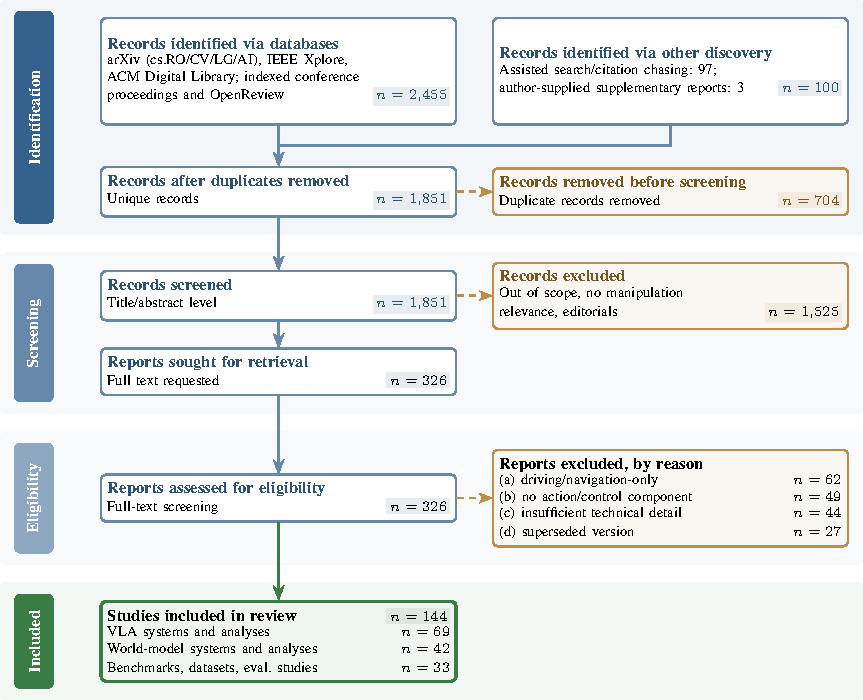
\includegraphics{figures/prisma.pdf}
\caption{PRISMA-style identification, screening, and selection diagram, including three author-supplied reports verified and included on 2~October~2026. The 100 records from other discovery comprise the original 97 assisted-search/citation-chasing records and these three additions. The final corpus contains 144 distinct papers: 69 VLA, 42 world-model, and 33 benchmark, dataset, or evaluation papers. The author-confirmed screening totals reconcile as 326 assessed = 182 excluded + 144 included; the included total matches the literature register.}
\label{fig:prisma}
\end{figure*}

\section{Literature Selection and Search Criteria}
\label{sec:methodology}

This section summarizes the search and selection process used to identify the literature reviewed in this article. A PRISMA-style procedure~\cite{prisma2020} was followed to identify relevant studies and apply consistent screening criteria (Fig.~\ref{fig:prisma}). \textcolor[RGB]{104,48,148}{The following subsections state the research questions, search scope, eligibility criteria, screening responsibilities, and the basis and limitations of the evidence synthesis.}

\subsection{Research Questions}
\label{sec:rq}

The review addresses four research questions:

\begin{enumerate}
\item[\textbf{RQ1:}] Which VLA systems have been proposed for robotic manipulation, and what problems do they address?
\item[\textbf{RQ2:}] What limitations and evaluation gaps are documented in current VLA research?
\item[\textbf{RQ3:}] Which world-model mechanisms are relevant to these limitations, and how directly are their effects supported?
\item[\textbf{RQ4:}] Under which evaluation protocols can results be compared, and where does the evidence remain incomplete?

\end{enumerate}

\subsection{Search Strategy}
\label{sec:search}

The search covered arXiv, IEEE Xplore, the ACM Digital Library, OpenReview, and proceedings from CoRL, ICRA, IROS, RSS, NeurIPS, ICLR, and CVPR. Curated research lists and benchmark leaderboards were used as additional discovery sources. The search window extended from January 2023 to August 2026 for VLA reports and from January 2018 to August 2026 for world models and evaluation resources. Earlier model-based control research was used for historical context but was not systematically screened. \textcolor[RGB]{104,48,148}{Targeted supplementary searches and reconciliation of the manuscript tables with the literature register were completed through 1~October~2026; three further author-supplied reports were verified and included on 2~October~2026.}

Two primary query families were used, with syntax adapted to each database:

\begin{quote}
\small
\textbf{VLA query:} (`vision-language-action'' OR `VLA model'' OR `robot foundation model'' OR `generalist robot policy'') AND (manipulation OR grasping OR ``mobile manipulation'')

\textbf{World-model query:} (`world model'' OR `video prediction'' OR `latent dynamics'' OR `JEPA'' OR `world foundation model'' OR `world-action model'' OR `world action model'' OR `world-action foundation model'' OR ``WAM'') AND (robot* OR manipulation OR embodied)
\end{quote}

Targeted searches were then conducted for topics not fully captured by the primary queries. These included action tokenization, flow-matching policies, predictive control, learned simulators, reinforcement-learning post-training, synthetic robot trajectories, physical-interaction prediction, and world-model evaluation. Forward and backward citation searches were performed from included surveys and influential systems.

Web-enabled ChatGPT and Claude were also used to support literature discovery. The same prompts were submitted to both systems. Representative prompts included:
 ``List vision-language-action models for robotic manipulation published between January 2023 and August 2026.''
``Which world models have been applied to robotic manipulation or embodied control?''
``Find studies that combine a world model and a VLA policy within one architecture.''
``Identify benchmarks for language-conditioned manipulation and robustness evaluation.''
``Find studies that use world models for reinforcement-learning post-training or synthetic robot data generation.''
``List surveys of VLA models, world models, and world-action models for robotics.''

Language-model suggestions were used only for record identification. Each suggested publication was verified through an arXiv record or publisher page before screening. Unverifiable suggestions were discarded, and generated summaries were never used as evidence. Duplicate records were removed using DOI and arXiv identifiers, followed by normalized title and author matching. Superseded versions were consolidated.

The search was designed primarily to identify systems and evaluation resources. The analysis of VLA limitations therefore represents a structured synthesis within the mapped corpus rather than an exhaustive estimate of all reported failures.

\subsection{Eligibility Criteria}
\label{sec:eligibility}

The inclusion criterion was a single retrievable paper, preprint, or technical report. Reports were eligible if they presented a VLA system, a world model, a training method, a dataset, a benchmark, or an evaluation study relevant to robotic manipulation. Peer-reviewed studies and technically detailed preprints were included. Reports on closed industrial systems were also retained because of their influence on the field, but their evidence was identified as vendor-reported.

Reports were excluded when they focused only on autonomous driving or navigation, contained no action or control component, or lacked sufficient technical detail for extraction. When several versions described the same work, the most complete version was retained. Related versions were linked through a common system identifier.

\textcolor[RGB]{104,48,148}{The final included corpus contains 144 distinct research papers: 69 on VLA systems and analyses, 42 on world-model systems and analyses, and 33 on datasets, benchmarks, and evaluation. Each paper is assigned one primary category for counting, with secondary roles retained for hybrid contributions. Background references and non-paper technical or software sources are recorded separately and are not included in this total.}

\subsection{Study Selection and Extraction}
\label{sec:selection-extraction}
\textcolor[RGB]{104,48,148}{Screening and extraction responsibilities were divided between reviewers across the VLA and world-model/benchmark corpora. This arrangement is not independent duplicate screening. The included-report register links each report to its title, year, primary source, summary, category, and inclusion decision. Reports are counted once even when they contribute to both policy learning and prediction. The final flow comprises 326 reports assessed for eligibility and 182 exclusions: 62 driving/navigation-only reports, 49 without an action/control component, 44 with insufficient technical detail, and 27 superseded versions. The remaining 144 reports match the included rows in the register.}

\textcolor[RGB]{104,48,148}{For quantitative comparisons, extraction retains the evaluated task and domain, observation and action configuration, baseline, training-data scope, reported outcome, uncertainty information, and source locator where available. A reported change is interpreted for the intervention actually compared, including a complete training or planning package when its components were not isolated. Source-reported values are not treated as matched comparisons merely because they share a benchmark name.}

\textcolor[RGB]{104,48,148}{The available review records do not provide an independent double-coding audit, agreement statistic, or a case-level disagreement log. The literature register also does not contain a complete report-by-report coding of every limitation and mechanism. These omissions limit reproducibility and prevent estimating the prevalence of each limitation across the 144-report corpus. No agreement coefficient or corpus-wide limitation frequency is inferred from citation counts.}

\subsection{Synthesis Framework and Interpretation}
\label{sec:synthesis-rubric}
\textcolor[RGB]{104,48,148}{The six limitation categories were organized around policy execution, transfer, training data, physical interaction, evaluation, and assurance during the narrative synthesis. No prespecified inductive coding scheme or independent category-development exercise is documented. They are analytical questions: execution monitoring and recovery (L1), distribution shift (L2), data requirements (L3), physical grounding (L4), evaluation validity (L5), and safety and uncertainty (L6). They are not mutually exclusive diagnoses of every VLA policy. Prediction and search latency are discussed separately as costs introduced by predictive mechanisms. The framework distinguishes failures or gaps documented for policies from hypotheses about how a world model might address them.}

\textcolor[RGB]{104,48,148}{Mechanism-effect statements are interpreted at the level of a specific claim and experiment. Direct evidence compares the claimed intervention or complete package with an identified baseline and measures the stated outcome under the reported protocol. It does not establish the contribution of an unablated component. Indirect evidence concerns a different outcome, domain, intervention, or unmatched comparison. Prospective connections have no corresponding empirical test in the cited report. Adverse denotes an unfavorable result or a failure of the proposed mechanism; it describes outcome direction and can coexist with direct or indirect evidence. These descriptions are an explicit interpretation rubric for the revised synthesis, not a retrospectively claimed independent coding exercise or a formal certainty grade.}

\textcolor[RGB]{104,48,148}{The 97 records in the assisted-discovery branch combine language-model suggestions and citation chasing. They cannot be attributed to either route separately from the retained count alone. Three additional author-supplied records---Seer, Video Prediction Policy, and Unified World Models---were verified against primary sources and included on 2~October~2026, giving 100 records in the combined other-discovery branch~\cite{seer,vpp,uwm}. Exact model versions, query dates, per-query yields, and discard counts are not documented in the available audit materials. Accordingly, the prompts above describe discovery examples rather than a fully reproducible search run. No reproducible Scopus or Web of Science search is claimed, and coverage beyond the listed sources remains a limitation.}



% Diagram source: tkz/vla-anatomy.tex.
% Fig — Anatomy of a VLA with two decoder families and a hierarchical wrapper.
\begin{figure*}[!t]
\centering
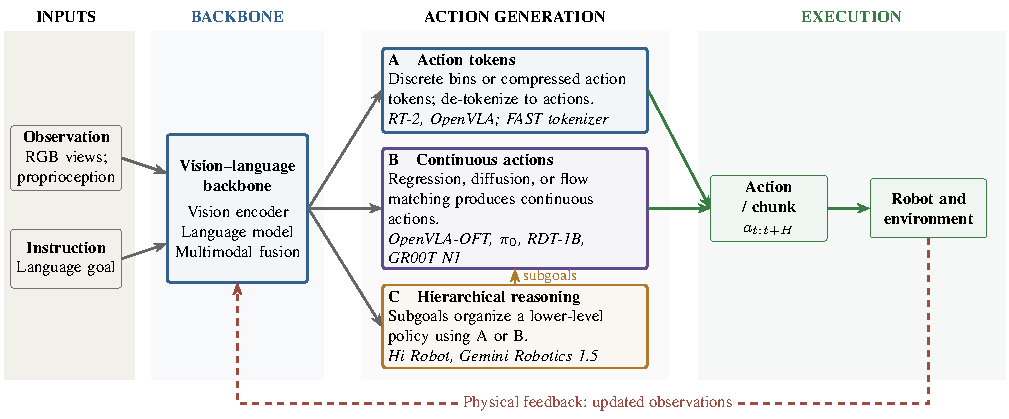
\includegraphics[width=0.95\linewidth]{figures/vla-anatomy.pdf}
\caption{\textcolor[RGB]{104,48,148}{A common, but not universal, VLA interface. Visual observations and language enter a vision--language backbone. Actions may be represented as discrete tokens (A) or continuous outputs generated through regression, diffusion, or flow matching (B). Hierarchical reasoning (C) can organize either action representation. The displayed systems are examples; the diagram does not imply a shared inference rate or an explicit candidate-action planner.}}
\label{fig:vla-anatomy}
\end{figure*}


\section{Vision-Language-Action Models}
\label{sec:vla}

Vision-language-action (VLA) models connect visual perception and language understanding with robot control. Most systems adapt a pretrained vision-language backbone to predict robot actions, although the specific representation and training strategy vary substantially. Fig.~\ref{fig:vla-anatomy} illustrates a common architecture in which visual observations and instructions are processed by a shared backbone before being passed to an action decoder.

The field cannot be described through a single architectural hierarchy. Some methods differ in how actions are represented, while others modify the training process or target a particular embodiment. We therefore organize the literature into seven overlapping groups according to the primary manipulation challenge addressed by each line of work. Fig.~\ref{fig:vla-taxonomy} summarizes this organization, and Table~\ref{tab:vla-master} provides a broader comparison. The groups are interpretive categories rather than mutually exclusive classes.

% ---- inlined from figs/fig_vla_taxonomy.tex ----
% Fig — VLA taxonomy tree, Groups A–G. Double column.
\begin{figure*}[!t]
\centering
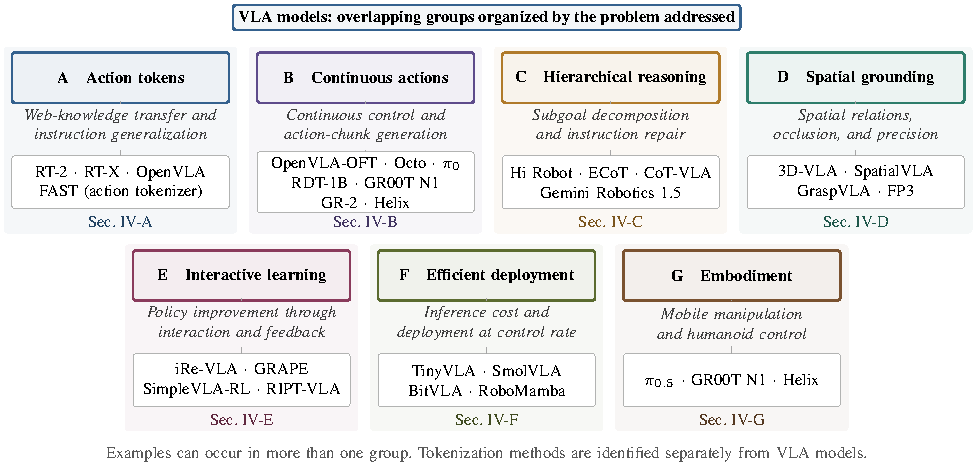
\includegraphics[width=0.95\linewidth]{figures/vla-taxonomy.pdf}
\caption{\textcolor[RGB]{104,48,148}{Problem-oriented VLA taxonomy with overlapping groups A--G and representative systems. The groups describe action representation, hierarchical reasoning, spatial grounding, interactive learning, efficient deployment, and embodiment. FAST is identified as a tokenizer rather than a standalone VLA.}}
\label{fig:vla-taxonomy}
\end{figure*}

\subsection*{Representative VLA Architecture}
\textcolor[RGB]{104,48,148}{Figure~\ref{fig:vla-detailed} expands the representative policy interface into perception, conditioning, action generation, and execution. Visual encoders transform one or more camera observations into features; language tokens express the task. A multimodal backbone combines these inputs with optional proprioception and temporal context. The resulting representation conditions an action head, whose output must be interpreted in the robot's declared action space, such as end-effector increments, joint targets, or gripper commands. These choices differ across systems~\cite{rt2,openvla,pi0}.}

\begin{figure*}[!t]
\centering
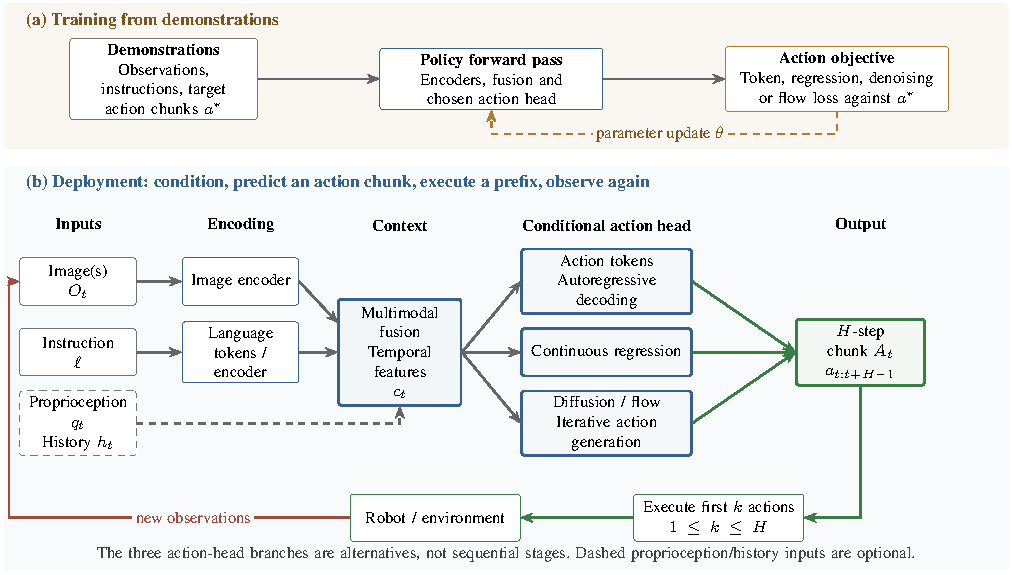
\includegraphics[width=0.99\linewidth]{figures/vla-detailed-architecture.pdf}
\caption{\textcolor[RGB]{104,48,148}{Representative VLA policy architecture. Perception and task conditioning feed an action generator, followed by chunk execution and observation feedback. Autoregressive tokens, direct continuous regression, and conditional diffusion/flow matching are alternative action-head designs, not mandatory sequential stages~\cite{rt2,openvla,openvlaoft,pi0}. Dashed proprioception/history inputs are optional; the dashed amber training arrow denotes parameter updates. The training and deployment paths distinguish learning from demonstrations from executing the resulting policy.}}
\label{fig:vla-detailed}
\end{figure*}

\textcolor[RGB]{104,48,148}{For a chunked policy, a representative interface is}
\begin{equation}
\color[RGB]{104,48,148}
A_t=(a_t,\ldots,a_{t+H-1})\sim\pi_\theta(\,\cdot\mid O_t,\ell,q_t,h_t),
\label{eq:vla-interface}
\end{equation}
\textcolor[RGB]{104,48,148}{where $O_t$ contains the available visual observations, $\ell$ is the language instruction, $q_t$ denotes optional measured proprioception, and $h_t$ denotes optional history. The notation includes deterministic policies as a limiting case and does not require a separate memory module. Token-based heads discretize actions and decode them autoregressively, while regression heads predict continuous values directly. Diffusion and flow-matching heads generate continuous actions through conditional iterative updates. OpenVLA-OFT's continuous regression and $\pi_0$'s flow matching therefore occupy different implementations of the same action-generation interface~\cite{openvla,openvlaoft,pi0}.}

\textcolor[RGB]{104,48,148}{Training uses observation--instruction--action examples and a loss matched to the output representation: token likelihood, regression error, or a diffusion/flow objective. Predictive auxiliary losses are optional. At deployment, a controller may execute the first $k\leq H$ actions ($H=k=1$ for a single-action interface) before acquiring new observations and querying the policy again; asynchronous implementations can overlap prediction and execution. Neither action-chunk duration nor actuator frequency equals complete observation-to-command latency. Feedback permits closed-loop correction, but its effectiveness must be measured through the recovery tests in Section~\ref{sec:l1}.}

\subsection{Group A: Action Tokens}
\label{sec:groupA}

Early VLA research focused on transferring semantic knowledge from vision-language models to robotic control. RT-1 established a transformer policy with discretized action bins~\cite{rt1}. RT-2 extended this approach by representing robot actions as text tokens and jointly training on web-scale visual-language data and robot trajectories~\cite{rt2}. This formulation allowed knowledge of objects and semantic concepts to influence action prediction.

The Open X-Embodiment initiative expanded this idea across multiple robotic platforms~\cite{oxe}. OpenVLA subsequently provided an open implementation based on fused visual encoders and a large language backbone~\cite{openvla}. Related systems explored alternative multimodal prompting and lighter adaptation strategies~\cite{vima,roboflamingo,llarva}. LAPA further reduced dependence on labeled robot actions by learning latent action representations from video~\cite{lapa}.

Later work addressed limitations of sequential token decoding. FAST introduced a frequency-space tokenizer for efficient action-sequence representation~\cite{fast}. \textcolor[RGB]{104,48,148}{Discrete-diffusion methods use iterative refinement to accelerate token generation~\cite{ddvla}. OpenVLA-OFT replaces token classification with continuous regression and is therefore discussed in Group~B.} These developments improve control resolution and efficiency, but the underlying policy still predicts actions directly. It does not explicitly model how alternative actions would change the environment.

\subsection{Group B: Continuous Actions}
\label{sec:groupB}

Continuous-action models address the precision and control-rate limitations of discrete tokenization. They commonly use diffusion or flow matching to generate smooth action sequences. This approach is particularly suitable for dexterous and bimanual manipulation, where several valid trajectories may satisfy the same instruction.

\textcolor[RGB]{104,48,148}{OpenVLA-OFT uses parallel continuous action prediction with an $\ell_1$ regression objective~\cite{openvlaoft}.} Octo demonstrated an open generalist policy with a diffusion decoder trained on Open X-Embodiment data~\cite{octo}. The $\pi_0$ architecture paired a vision-language backbone with a flow-matching action expert~\cite{pi0}. RDT-1B used a diffusion transformer and a unified action space to support heterogeneous embodiments~\cite{rdt1b}. CogACT and DexVLA similarly separated semantic reasoning from continuous control through specialized action modules~\cite{cogact,dexvla}. These designs build on action chunking and diffusion-based control developed in earlier imitation-learning systems~\cite{act,mobilealoha,diffusionpolicy}.

The same pattern appears in larger robotic foundation models. GR00T~N1 combines a vision-language module with a diffusion action head for humanoid control~\cite{groot}. The $\pi_{0.5}$ model extends continuous action generation to mobile manipulation and long-duration tasks~\cite{pi05}. Closed systems such as Gemini Robotics and Figure Helix follow related dual-system designs but remain vendor-reported~\cite{geminirobotics,helix}.

Action chunking reduces repeated policy computation, but longer chunks also delay feedback. \textcolor[RGB]{104,48,148}{Action-execution frequency, policy-query rate, and planning latency are distinct quantities. For example, $\pi_0$ reports 50-Hz action execution, while GR00T~N1 reports inference latency for a multi-action chunk~\cite{pi0,groot}. The action-head design alone does not establish recovery or the benefit of candidate-action planning.}

\textcolor[RGB]{104,48,148}{Predictive policies also use continuous action heads. Seer conditions inverse dynamics on forecast visual states, while Video Prediction Policy (VPP) uses predictive video representations with a diffusion policy head~\cite{seer,vpp}. Both first appeared in December 2024, preceding WorldVLA, and connect the policy taxonomy to the predictive mechanisms in Section~\ref{sec:wm6}.}

\subsection{Group C: Hierarchical Reasoning}
\label{sec:groupC}

Long-horizon manipulation requires more than accurate local control. A robot must identify intermediate goals and recover when execution departs from the intended plan. Hierarchical methods address this problem by separating high-level deliberation from low-level action generation.

Early systems established several forms of this separation. SayCan grounded language-model plans using learned value functions~\cite{saycan}. PaLM-E incorporated continuous observations into an embodied language model~\cite{palme}, while RT-H introduced a language-motion hierarchy between instructions and actions~\cite{rth}. Code as Policies and VoxPoser used generated programs or spatial value maps as interfaces between reasoning and control~\cite{codeaspolicies,voxposer}.

More recent VLAs integrate reasoning more directly with action prediction. Hi Robot places an open-vocabulary policy above a continuous executor~\cite{hirobot}. ECoT generates intermediate reasoning before actions~\cite{ecot}, while OneTwoVLA switches between reasoning and execution according to the task context~\cite{onetwovla}. RationalVLA introduces feasibility reasoning for rejecting unsuitable instructions~\cite{rationalvla}. ReKep and MOKA use visual keypoints or marked images to connect semantic reasoning with geometric control~\cite{rekep,moka}.

CoT-VLA is especially relevant to the predictive direction of this review because its reasoning process includes predicted future frames~\cite{cotvla}. However, a single anticipated future does not provide systematic comparison among alternative actions. More broadly, learned hierarchical policies do not normally offer the feasibility guarantees or backtracking mechanisms associated with task-and-motion planning~\cite{ontollmtamp}. Their main contribution is improved task organization, while verified consequence reasoning remains open.

\subsection{Group D: Spatial Grounding}
\label{sec:groupD}

VLA models built mainly on two-dimensional images can struggle with metric placement and viewpoint changes. Spatially grounded methods address this limitation by incorporating depth, point clouds, voxels, or learned three-dimensional features.

PerAct and RVT established the value of voxel and multi-view representations for precise manipulation~\cite{peract,rvt}. Later systems improved the efficiency and accuracy of these representations~\cite{rvt2,act3d}. Within the VLA paradigm, 3D-VLA connected a three-dimensional language model with diffusion-based action generation~\cite{threedvla}. SpatialVLA encoded egocentric geometry as spatial action tokens~\cite{spatialvla}, while PointVLA incorporated point clouds into a pretrained VLA~\cite{pointvla}. Lift3D and FP3 transferred foundation-model features into three-dimensional policy representations~\cite{lift3d,fp3}.

Other systems combine semantic priors with task-specific geometric interfaces. BridgeVLA aligns vision-language features with spatial heatmaps~\cite{bridgevla}, and GraspVLA uses large-scale synthetic grasp data to support spatially grounded grasping~\cite{graspvla}. GeoVLA and 3D-CAVLA further integrate geometric encoders with contextual reasoning~\cite{geovla,cavla}.

These methods improve knowledge of where objects and targets are located. This is not equivalent to learning how objects will move or deform under contact. Spatial grounding strengthens the state representation, whereas consequence prediction requires a model of dynamics.

\subsection{Group E: Interactive Learning}
\label{sec:groupE}

Supervised VLA policies inherit the coverage of their demonstrations. When execution moves outside that coverage, the policy may lack corrective or recovery behavior. Reinforcement-learning post-training addresses this limitation through interaction and task-level feedback.

Several methods combine reinforcement learning with supervised stabilization. iRe-VLA alternates online improvement with supervised consolidation~\cite{irevla}. GRAPE uses trajectory-level preferences~\cite{grape}, while RLDG transfers skills from specialist reinforcement-learning policies into a generalist VLA~\cite{rldg}. ConRFT applies reinforced fine-tuning on physical robots~\cite{conrft}, and VLA-RL scales policy optimization using learned progress signals~\cite{vlarl}.

Recent studies report substantial gains in particular LIBERO configurations. SimpleVLA-RL improves an OpenVLA-OFT starting point through online interaction~\cite{simplevlarl}, while RIPT-VLA uses sparse rewards to improve a weak supervised policy~\cite{riptvla}. FLaRe also reports generalization gains from large-scale reinforcement-learning adaptation~\cite{flarerl}. These results show that supervised policies can be improved through interaction. They do not establish whether the benefit comes from reinforcement learning alone because the data distribution and feedback signal also change.

The practical limitation is that physical interaction is expensive and may be unsafe. Conventional simulators provide one solution, while learned world models offer another. The latter could extend interactive training beyond available demonstrations, but their value depends on whether improvements obtained in the learned environment transfer to the real robot.

\subsection{Group F: Efficient Deployment}
\label{sec:groupF}

On-robot deployment imposes strict limits on memory and inference time. Efficiency research reduces these costs through smaller backbones, alternative sequence models, compressed weights, and faster decoding.

TinyVLA and SmolVLA show that compact policies can retain competitive task performance~\cite{tinyvla,smolvla}. EdgeVLA further adapts non-autoregressive action prediction to embedded hardware~\cite{edgevla}. RoboMamba replaces standard attention with state-space dynamics~\cite{robomamba}, while BitVLA combines low-bit weights with vision compression~\cite{bitvla}. Other methods exploit temporal redundancy or prune unnecessary computation~\cite{vlacache,efficientvla}.

Decoding can also be adapted to the difficulty of the current situation. PD-VLA and CEED-VLA accelerate action generation through parallel prediction or early exit~\cite{pdvla,ceedvla}. DeeR-VLA applies adaptive exits within the multimodal backbone~\cite{deervla}. Gemini Robotics On-Device represents a closed implementation of the same deployment objective~\cite{geminiondevice}.

Efficiency is not only a hardware concern. Reducing policy cost can support more frequent replanning or release computation for uncertainty estimation and predictive search. However, a faster policy is not necessarily more reliable. The key question is whether saved computation can be converted into better closed-loop reasoning within the available control deadline.

\subsection{Group G: Embodiment}
\label{sec:groupG}

Moving beyond tabletop manipulation introduces mobile bases, whole-body motion, and humanoid platforms. These embodiments increase the state dimension and amplify the consequences of planning errors.

OWMM-Agent combines scene understanding with navigation and grasping in a mobile manipulation system~\cite{owmmagent}. OK-Robot examines how open components can support manipulation in unfamiliar homes~\cite{okrobot}. The $\pi_{0.5}$ model extends a generalist policy to mobile manipulation over long task sequences~\cite{pi05}, while Long-VLA and LoHoVLA address error accumulation across extended execution horizons~\cite{longvla,lohovla}.

Humanoid systems further require coordination across the upper body or the entire platform. GR00T~N1 and N1.5 provide open foundation models for humanoid control~\cite{groot,grootn15}. Figure Helix demonstrates high-rate upper-body control on commercial hardware, although its results remain closed and vendor-reported~\cite{helix}. These systems broaden the scope of VLA policies, but evidence across platforms remains difficult to compare because embodiments and evaluation protocols differ substantially.

As the platform becomes more capable, the cost of an incorrect action also increases. Embodiment scaling therefore strengthens the case for predictive evaluation and runtime assurance rather than serving only as another measure of policy generality.

\medskip
\noindent\textbf{Summary.}
The seven groups capture complementary responses to the central challenges of VLA-based manipulation. Action-token and continuous-action models improve semantic transfer and motor generation. Hierarchical and spatially grounded systems extend reasoning and representation. Interactive learning addresses weaknesses inherited from supervised data, while efficiency and embodiment research target deployment constraints. \textcolor[RGB]{104,48,148}{These advances blur the boundaries between categories. The next section considers behavioral and evaluation questions that apply to both direct policies and predictive systems, without treating a missing architectural component as a failure by itself.}


% Table II — Representative VLA systems by group (compact master table)
\begin{table*}[!t]
\caption{Representative vision-language-conditioned manipulation policies
and VLA-based systems by problem-oriented group. Standalone language planners,
embodied VLMs without an action policy, and navigation-only systems are excluded.
Groups may overlap; year denotes the first public report. Action: AR =
autoregressive, Diff = diffusion, FM = flow matching, Hier = hierarchical.
Open: \cmark~= official public code or weights, (\cmark)~= only part of the model family or artifacts released,
--- = no verified release.
$^{\dagger}$Pre-2023 language-conditioned action-policy precursor.
Headline results use each source's protocol and are not comparable across rows.}
\label{tab:vla-master}
\centering
\scriptsize
\setlength{\tabcolsep}{3.5pt}
\begin{tabular}{p{2.5cm}p{0.7cm}p{0.7cm}p{2.2cm}p{2.0cm}p{0.7cm}p{5.5cm}}
\toprule
Model & Year & Grp & Backbone & Action head & Open & Headline (source protocol) \\
\midrule
RT-1$^{\dagger}$~\cite{rt1} & 2022 & A & EfficientNet + Transformer & Parallel action bins & \cmark & Language-conditioned control; 130k episodes \\
RT-2~\cite{rt2} & 2023 & A & PaLI-X/PaLM-E (55B) & AR text tokens & --- & Emergent semantic generalization \\
RT-X~\cite{oxe} & 2023 & A & RT-1 / RT-2 & Discrete / AR tokens & (\cmark) & Cross-embodiment transfer; RT-1-X checkpoint released \\
OpenVLA~\cite{openvla} & 2024 & A & Llama-2-7B & AR bins & \cmark & +16.5 percentage points over RT-2-X (55B) \\
FAST / $\pi_0$-FAST~\cite{fast} & 2025 & A & PaliGemma-3B & AR (DCT tokens) & \cmark & AR at dexterous control rates \\
OpenVLA-OFT~\cite{openvlaoft} & 2025 & \textcolor[RGB]{104,48,148}{B} & Llama-2-7B & Parallel cont.\ ($\ell_1$ loss) & \cmark & LIBERO 95.3\% or 97.1\%, config.-specific \\
\textcolor[RGB]{104,48,148}{Seer~\cite{seer}} & \textcolor[RGB]{104,48,148}{2024} & \textcolor[RGB]{104,48,148}{B} & \textcolor[RGB]{104,48,148}{GPT-2-style transformer} & \textcolor[RGB]{104,48,148}{MLP inverse dynamics} & \textcolor[RGB]{104,48,148}{\cmark} & \textcolor[RGB]{104,48,148}{Forecast visual states condition manipulation actions} \\
\textcolor[RGB]{104,48,148}{VPP~\cite{vpp}} & \textcolor[RGB]{104,48,148}{2024} & \textcolor[RGB]{104,48,148}{B} & \textcolor[RGB]{104,48,148}{Video diffusion + Video Former} & \textcolor[RGB]{104,48,148}{Diffusion policy} & \textcolor[RGB]{104,48,148}{\cmark} & \textcolor[RGB]{104,48,148}{Predictive visual features for simulated and physical manipulation} \\
Octo~\cite{octo} & 2024 & B & Transformer (27M/93M) & Diff chunks & \cmark & 800k OXE episodes; language/image goals \\
$\pi_0$~\cite{pi0} & 2024 & B & PaliGemma-3B+300M & FM chunks; 50-Hz execution & \cmark & 10k+ h teleop, 7 platforms \\
RDT-1B~\cite{rdt1b} & 2024 & B & 1.2B DiT & Diff chunks & \cmark & 1M+ pretraining episodes; 6k+ ALOHA fine-tuning episodes \\
GR00T N1~\cite{groot} & 2025 & B & Eagle-2 (1.34B) & DiT FM, dual-sys & \cmark & 16-act chunk / 63.9\,ms (L40) \\
GR00T N1.7~\cite{grootn17} & 2026 & B/G & Cosmos-Reason2-2B & DiT FM chunks & \cmark & Open 3B cross-embodiment policy \\
$\pi_{0.5}$~\cite{pi05} & 2025 & B/G & PaliGemma-class 4B & FM + high-level & \cmark & Unseen-home mobile cleaning \\
$\pi_{0.7}$~\cite{pi07} & 2026 & B/C & Gemma3-4B + 860M expert & FM + multimodal prompts & --- & Language/subgoal steering; cross-embodiment transfer \\
LingBot-VLA 2.0~\cite{lingbotvla2} & 2026 & B/D/G & Qwen3-VL-4B + MoE & FM; 55-D actions & \cmark & Whole-body actions; future-feature supervision \\
GR-2~\cite{gr2} & 2024 & B & Video transformer (230M) & cVAE action chunks & --- & 97.7\% over 105 internal tabletop tasks \\
Gemini Robotics~\cite{geminirobotics} & 2025 & B & Gemini 2.0 & Closed & --- & Frontier dexterity (vendor) \\
Helix~\cite{helix} & 2025 & B/G & 7B S2 + 80M S1 & Dual-sys, 200\,Hz & --- & Whole-upper-body humanoid \\
Helix 02~\cite{helix02} & 2026 & B/G & S2 + S1 + learned S0 & Joint targets + whole-body ctrl. & --- & Continuous loco-manipulation with tactile input \\
Hi Robot~\cite{hirobot} & 2025 & C & PaliGemma-3B + $\pi_0$ & Hier + FM chunks & --- & Hierarchical reasoning with a learned VLA executor \\
ECoT~\cite{ecot} & 2024 & C & OpenVLA-base & AR + reasoning & \cmark & +CoT before acting \\
CoT-VLA~\cite{cotvla} & 2025 & C & VILA-U (7B) & AR frames + action chunks & --- & Predicted visual subgoals guide closed-loop actions \\
LoHoVLA~\cite{lohovla} & 2025 & C & PaliGemma-3B & AR language + actions & --- & 20 long-horizon Ravens tabletop tasks \\
Gemini Robotics 1.5~\cite{gemini15} & 2025 & C & Gemini + ER 1.5 & Hier, thinking & --- & Interleaved reasoning, motion transfer \\
3D-VLA~\cite{threedvla} & 2024 & D & 3D-LLM & Diff (3D) & \cmark & 3D world-model-style heads \\
SpatialVLA~\cite{spatialvla} & 2025 & D & PaliGemma2-3B & Spatial AR tokens & \cmark & 4B policy; 1.1M real-robot episodes \\
GraspVLA~\cite{graspvla} & 2025 & D & InternLM2 + vision & AR perception + FM & \cmark & Billion-frame synthetic grasp data; open-vocabulary grasping \\
FP3~\cite{fp3} & 2025 & D & Uni3D + CLIP + DiT & Diff chunks & \cmark & Language-conditioned 3D policy; 60k DROID episodes \\
SimpleVLA-RL~\cite{simplevlarl} & 2025 & E & Modified OpenVLA-OFT & Parallel action tokens & \cmark & Online RL; LIBERO and RoboTwin evaluations \\
RIPT-VLA~\cite{riptvla} & 2025 & E & QueST / OpenVLA-OFT & AR / continuous chunks & \cmark & RL post-training with sparse success rewards \\
FLaRe~\cite{flarerl} & 2024 & E & SPOC transformer & Discrete actions & \cmark & PPO tuning; 79.5\% CHORES-S (simulated navigation/manipulation) \\
TinyVLA~\cite{tinyvla} & 2024 & F & Compact VLM family & Diff & \cmark & 0.4--1.3B family; no robot pretraining \\
SmolVLA~\cite{smolvla} & 2025 & F & SmolVLM2 + expert & FM & \cmark & 450M policy; consumer-GPU training \\
BitVLA~\cite{bitvla} & 2025 & F & BitNet-2B + SigLIP & Parallel cont.\ MLP & \cmark & Ternary-weight backbone; OFT-style action regression \\
RoboMamba~\cite{robomamba} & 2024 & F & CLIP + Mamba-2.7B & MLP pose regression & (\cmark) & Efficient pose prediction; training code by request \\
\bottomrule
\end{tabular}
\end{table*}

\section{Limits of Current VLA Systems}
\label{sec:limitations}

\textcolor[RGB]{104,48,148}{This section examines six evaluation questions for VLA-based manipulation: execution monitoring and recovery, distribution shift, data requirements, physical grounding, evaluation validity, and safety and uncertainty. These questions concern observable behavior and experimental support, rather than the presence of a particular architecture. A policy need not contain an explicit world model to address them. Table~\ref{tab:matrix} separates evidence for each limitation from evidence that a predictive mechanism improves the relevant outcome. The computational cost of prediction and search is discussed separately in Section~\ref{sec:wmweak}.}

\subsection{L1: Execution Monitoring and Recovery}
\label{sec:l1}
\textcolor[RGB]{104,48,148}{Successful nominal execution does not establish whether a policy detects an unsuccessful action and corrects it before continuing. Relevant outcomes include recovery after a failed grasp or misplaced object, the time needed to detect the error, and repeated execution of ineffective actions. This is a behavioral question: both direct policies and predictive systems can be evaluated under the same controlled failure interventions.}

\textcolor[RGB]{104,48,148}{Recent VLA work treats recovery as a distinct capability. The $\pi_0$ training discussion explicitly motivates retaining corrective behavior~\cite{pi0}, while ReCoVLA evaluates failure detection and residual correction around frozen VLA policies~\cite{recovla}. These studies do not establish that all VLAs fail to recover, or that a world model is required. They motivate reporting recovery separately from aggregate task success.}

\textcolor[RGB]{104,48,148}{WorldVLA reports qualitative re-grasping examples and policy-success ablations, whereas Cosmos Policy compares a refined planning package with direct execution~\cite{worldvla,cosmospolicy}. These results support their respective implementations, but aggregate completion does not isolate detection or recovery after a controlled execution error. For L1, they provide indirect evidence; a matched recovery comparison remains an evaluation gap in these selected examples.}

\subsection{L2: Distribution Shift}
\label{sec:l2}
\textcolor[RGB]{104,48,148}{Distribution shift concerns transfer across changes in the task or observation distribution, including layouts, camera viewpoints, instructions, and embodiments. Unlike L1, which evaluates correction within an execution, L2 asks whether performance persists across declared changes to the deployment conditions. LIBERO-Plus provides direct evidence of sensitivity to controlled visual and initial-state perturbations in the policies it evaluates~\cite{liberoplus}; its language tests also caution that insensitivity to paraphrases can conceal failure to use the instruction. These findings are specific to the tested policies and protocols, rather than a universal limit on VLA generalization.}

Reinforcement-learning post-training can substantially improve particular supervised policies. SimpleVLA-RL, RIPT-VLA, and FLaRe report large gains after introducing interaction and reward feedback~\cite{simplevlarl,riptvla,flarerl}. However, these studies change the data distribution and optimization objective together. They therefore demonstrate that the original policies can be improved, but do not establish a universal performance ceiling for imitation learning. Dataset aggregation and interactive learning remain valid alternatives to world-model-based practice.

\subsection{L3: Data Requirements}
\label{sec:l3}

VLA models inherit broad visual and semantic knowledge from pretrained backbones, but grounding that knowledge in robot actions still requires expensive interaction data. The scale of current efforts illustrates this burden. The $\pi_0$ dataset contains more than 10{,}000 hours of teleoperation~\cite{pi0}, DROID contributes 350 hours of robot interaction~\cite{droid}, and Open X-Embodiment aggregates 970,000 trajectories across many institutions~\cite{oxe}.

Predictive systems can exploit larger collections of passive video. V-JEPA~2 uses extensive action-free video before action-conditioned adaptation~\cite{vjepa2}, while Dreamer~4 separates passive gameplay data from a smaller paired-action subset~\cite{dreamer4}. These examples show that passive data can support predictive representation learning. They do not quantify how many hours of robot interaction are replaced because the tasks and supervision differ. Fig.~\ref{fig:data-roles} therefore separates passive video from action-conditioned and robot-demonstration data.

\begin{figure*}[!t]
\centering
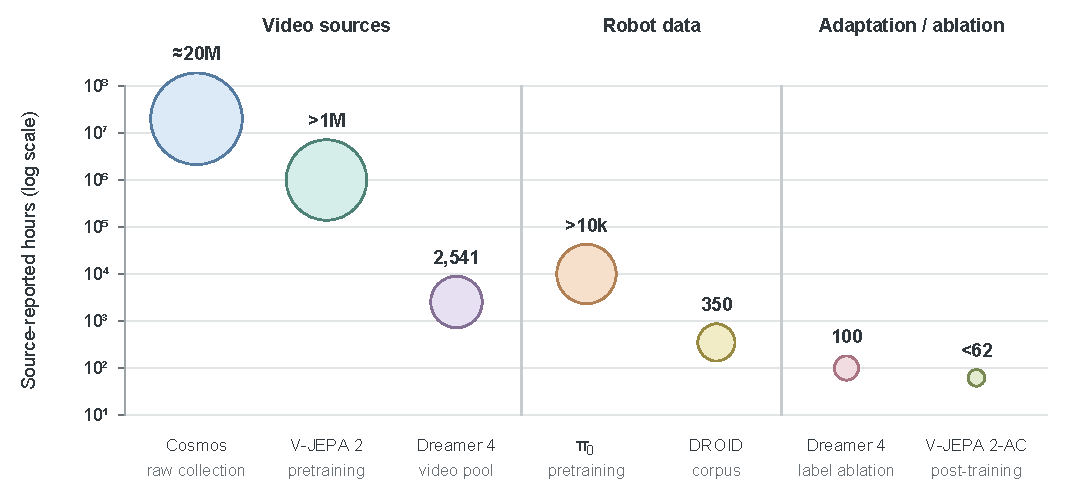
\includegraphics[width=0.97\linewidth]{figures/figure_06_data_scale_bubbles.pdf}
\caption{\textcolor[RGB]{104,48,148}{Source-reported data scales shown as light-filled bubbles on a logarithmic hours axis~\cite{cosmos,vjepa2,pi0,dreamer4,droid}. Colors distinguish the plotted records. Bubble area increases linearly with the logarithm of the reported value or bound threshold; areas are not proportional to raw hours. The numerical labels retain approximate values and lower or upper bounds. Cosmos denotes the raw candidate collection, $\pi_0$ a robot pretraining mixture, and DROID its reported demonstration corpus. Dreamer~4's 100-hour action-label generation ablation is nested within its 2,541-hour gameplay pool (90/10 training/evaluation split), not the full agent-training budget. V-JEPA~2-AC denotes robot-video post-training with states and derived actions, excluding earlier video pretraining. Different tasks, supervision, and populations prevent a sample-efficiency ranking.}}
\label{fig:data-roles}
\end{figure*}

\subsection{L4: Physical Grounding}
\label{sec:l4}

Visual plausibility does not guarantee correct physical behavior. A model may generate realistic images while misrepresenting contact or object dynamics. Geometric accuracy must also be distinguished from causal validity because knowing where an object is does not establish how it will respond to an action.

\textcolor[RGB]{104,48,148}{Physics-IQ evaluates video generators rather than VLA control. Its association between an MLLM distinguishability score and the physics score is not statistically significant ($r=-0.46$, $p=0.249$); this does not establish an absence of association~\cite{physicsiq}. Generator benchmarks therefore motivate physical-interaction tests, but do not demonstrate that the reviewed policies lack physical grounding.}

\textcolor[RGB]{104,48,148}{WorldModelBench and VBench-2.0 also expose physical inconsistencies in generated video~\cite{wmbench,vbench2}.}

Direct evaluation should vary physical properties while controlling visual appearance and then measure both prediction error and policy behavior. The main finding is therefore an evaluation gap rather than proof that current VLAs lack physical understanding.

\subsection{L5: Evaluation Validity}
\label{sec:l5}

Several VLA systems report near-saturated performance on standard LIBERO configurations~\cite{openvlaoft,simplevlarl,cosmospolicy}. However, LIBERO-Plus shows that performance can decline sharply under changes in viewpoint, layout, or language~\cite{liberoplus}. This contrast indicates that success on the original benchmark may not reflect robust instruction grounding or environmental generalization.

Simulation introduces another layer of uncertainty. PolaRiS shows that generated rollouts may contain hallucinated interactions and may not preserve real-world policy rankings~\cite{polaris}. SimplerEnv was developed to improve correspondence between simulation and physical evaluation~\cite{simplerenv}, but simulator performance still depends on the selected tasks and calibration procedure. Benchmark results should therefore be interpreted within their original protocols. A learned evaluator or larger simulator does not automatically provide valid real-world comparison.

\subsection{L6: Safety and Uncertainty}
\label{sec:l6}

Standard behavior-cloning objectives do not require calibrated uncertainty or estimates of constraint violation. They also do not identify when an action may cause irreversible harm. These capabilities must be introduced through the learning objective or through a separate assurance layer.

LIBERO-Safety evaluates policies in safety-critical manipulation settings~\cite{safelibero}, while ASIMOV accompanies the vendor-reported safety framework of Gemini Robotics~\cite{gemini15}. Other approaches use uncertainty to request assistance or abstain from unsupported actions~\cite{knowno}. Control barrier functions and reachability methods can provide runtime protection without a generative world model~\cite{cbf,hjreach}.

A world model may make predicted outcomes available for inspection, but prediction is neither necessary nor sufficient for safety. An inaccurate model can produce confident and unsafe forecasts. Consequence prediction must therefore be combined with uncertainty calibration, runtime enforcement, and a tested fallback policy.

\medskip
\noindent\textbf{Summary.}
\textcolor[RGB]{104,48,148}{The six questions distinguish policy behavior, training coverage, and the validity and assurance of evaluation. Their overlap should be recorded rather than interpreted as six independent failure modes. The next section examines predictive mechanisms that may address these questions and identifies the outcome actually measured by each selected comparison.}

% =========================================================================

\begin{figure*}[!t]
\centering
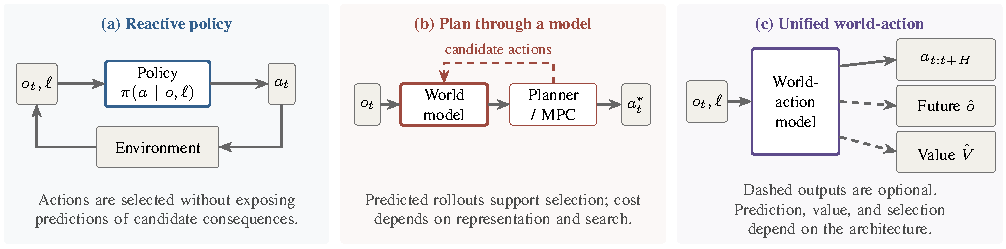
\includegraphics[width=0.95\linewidth]{figures/contrast.pdf}
\caption{Three control interfaces. (a)~A policy maps observations directly
to actions without exposing a consequence model. (b)~An explicit predictive
model permits candidate search, with cost determined by representation and
search. (c)~A unified model shares representations for predictive and action
objectives; future-state and value outputs are architecture-dependent and need
not be emitted during every direct-policy inference. Explicit best-of-$N$
selection still requires repeated queries and is not near-policy latency by default.}
\label{fig:contrast}
\end{figure*}

\section{World Models and Predictive Mechanisms}
\label{sec:wm}

World models extend robot learning beyond direct action prediction by learning how the environment changes over time. Their role varies across systems. Some support planning in a compact latent space, while others generate future observations or provide imagined experience for policy learning. More recent architectures combine prediction and action generation within a shared model (Fig.~\ref{fig:deepdives}).

\subsection{Scope and Taxonomy}
\label{sec:wmdef}

Under partial observability, a world model infers a state representation from the available observation and action history. The state is then propagated through an action-conditioned transition model:
\begin{equation}
z_t \sim q_\phi(z_t \mid h_t),
\qquad
p_\theta(z_{t+1} \mid z_t,a_t).
\end{equation}
The predicted state may be decoded into future observations or used to estimate task value and termination. Language can also condition the transition when the instruction changes which aspects of the environment are relevant.

This definition concerns model structure rather than downstream use. The same predictive model may support planning, imagined policy learning, synthetic data generation, or policy evaluation. We also include predictive components learned from passive video when an action-conditioned adaptation is provided. However, action conditioning alone does not establish causal validity. Reliable candidate comparison also requires sufficient state information and support for the evaluated actions.

The literature is organized into six overlapping families according to prediction space and functional role. The comparison in Fig.~\ref{fig:contrast} distinguishes direct policies from planning through a model and from unified world-action architectures. Fig.~\ref{fig:wm-taxonomy} summarizes the six families, while Table~\ref{tab:wm-master} provides representative systems. These categories are not mutually exclusive because a single model may serve several predictive functions.

% Retain the existing reactive, predictive, and unified comparison figure here.
% Retain the existing world-model taxonomy figure here.

\subsection*{Representative Action-Conditioned World Model}
\textcolor[RGB]{104,48,148}{Figure~\ref{fig:wm-detailed} depicts a representative world model for predictive control. An encoder and state estimator summarize observations and, where needed, action history. A transition model predicts the next internal state under a supplied action. Decoders can reconstruct observations or predict task outcomes; reward, termination, and uncertainty outputs depend on the architecture and training signals. This control-oriented interface is exemplified by latent-dynamics methods, while predictive representations and video-based systems instantiate different subsets of it~\cite{planet,dreamerv3,tdmpc2,vjepa2}.}

\begin{figure*}[!t]
\centering
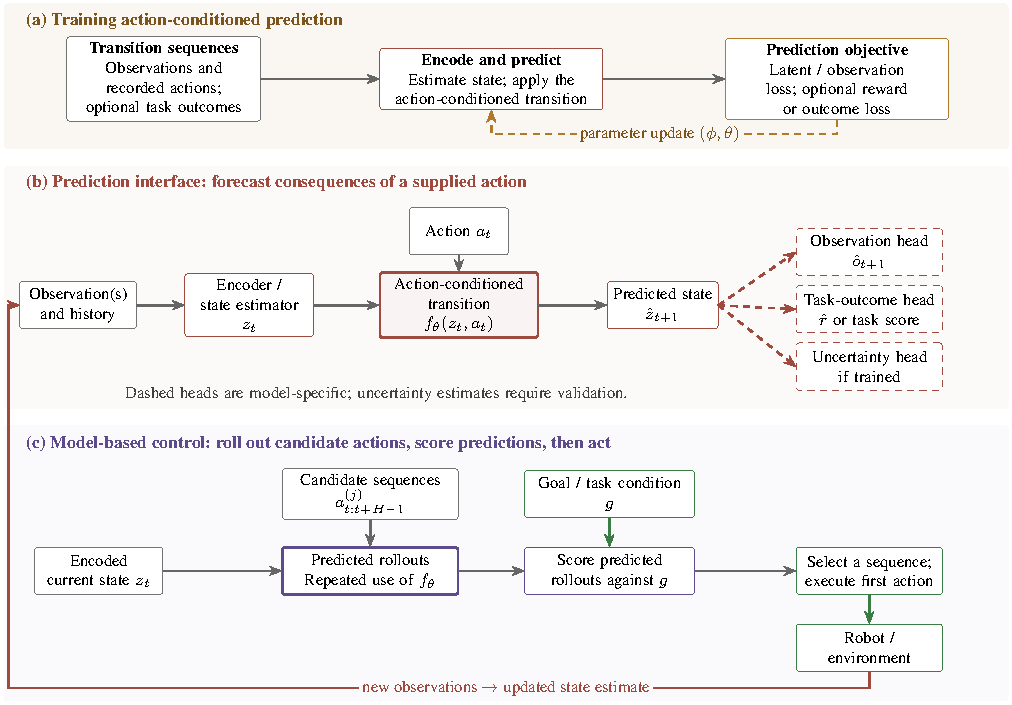
\includegraphics[width=0.99\linewidth]{figures/world-model-detailed-architecture.pdf}
\caption{\textcolor[RGB]{104,48,148}{Representative action-conditioned world model and its use in receding-horizon planning. State estimation, supplied-action transition prediction, and optional output heads form the model. A planner evaluates candidate action sequences using a task objective, executes an initial action or prefix, and updates from observations~\cite{planet,tdmpc2,vjepa2}. Training uses observed transitions; some architectures also learn rewards or termination. Dashed modules are optional. Learned uncertainty is not a safety certificate, and the diagram does not imply that all world-model families expose every interface.}}
\label{fig:wm-detailed}
\end{figure*}

\textcolor[RGB]{104,48,148}{A compact stochastic formulation is}
\begin{equation}
\color[RGB]{104,48,148}
z_t=E_\phi(o_{\leq t},a_{<t}),\qquad
\hat z_{t+1}\sim p_\theta(\,\cdot\mid z_t,a_t),
\label{eq:wm-interface}
\end{equation}
\textcolor[RGB]{104,48,148}{where $z_t$ summarizes the information used for prediction and need not be a fully observed physical state. Equation~\ref{eq:wm-interface} is one stochastic formulation; deterministic transitions $\hat z_{t+1}=f_\theta(z_t,a_t)$ and recurrent belief-state updates are also used. It does not require every predictor to define a normalized probability density. Goal or language conditioning may be added, but it does not replace the supplied action $a_t$. During training, observed transitions constrain prediction; objectives can target pixels, latent features, or task-relevant outcomes. Multi-step training may improve rollout consistency, yet prediction error can still accumulate beyond the training horizon. Passive video can support representation or generative pretraining, while identifying executable-action transitions requires appropriate action grounding.}

\textcolor[RGB]{104,48,148}{For online planning, candidate actions are repeatedly propagated through the transition model and scored against an external goal or learned task objective. The controller executes an initial action or prefix and re-estimates the state from new observations. Goal-distance planning need not learn a reward head, and a stochastic predictor need not provide calibrated epistemic uncertainty~\cite{vjepa2}. Alternatively, imagined rollouts can update an actor without online search at action selection, or predictive objectives can shape a policy without online search~\cite{dreamerv3,flarewm}. These are different uses of prediction. Action conditioning alone establishes neither causal identification nor safety; intervention tests, support checks, and runtime protection remain separate requirements.}

\subsection{WM1: Latent Dynamics}
\label{sec:wm1}

Latent-dynamics models learn a compact state in which future outcomes can be predicted without generating every image detail. This representation supports efficient planning and policy learning through imagined trajectories.

The recurrent World Models framework established the idea of training a policy inside a learned environment~\cite{worldmodels2018}. PlaNet later introduced practical planning with a recurrent state-space model~\cite{planet}. The Dreamer family replaced online search with actor-critic learning in imagination and demonstrated strong performance across diverse control domains~\cite{dreamerv3}. MuZero showed that a useful model need not reconstruct observations when it can predict quantities that matter for decisions~\cite{muzero}. TD-MPC2 further scaled latent planning across continuous-control tasks~\cite{tdmpc2}.

Dreamer~4 provides an important recent example of learning entirely inside a world model from offline data~\cite{dreamer4}. Its Minecraft result demonstrates that imagined learning can support complex behavior with limited action-labeled data. However, it remains a cross-domain proof of concept rather than direct evidence for general robotic manipulation. Latent dynamics offer a promising response to interaction cost and planning latency, but their benefit must still be established under physical contact and real-world distribution shift.

\subsection{WM2: Generative Video Models}
\label{sec:wm2}

Generative world models predict future observations in pixel space. Their main advantage is the ability to learn broad visual dynamics from large video collections and present predicted outcomes in an interpretable form.

UniPi formulated decision making as language-conditioned video generation followed by inverse dynamics~\cite{unipi}. UniSim extended video prediction toward interactive learned simulation~\cite{unisim}. Related work extracts actions from passive video or generates intermediate visual goals for control~\cite{avdc,susie,vlp,ivideogpt}. GR-1 and GR-2 brought video-predictive pretraining into manipulation policies~\cite{gr1,gr2}.

Large world foundation models extend this approach beyond individual tasks. Cosmos provides an open platform for video tokenization and generative dynamics~\cite{cosmos}. The Genie family focuses on interactive environments that respond to user control~\cite{genie1,genie3}. Genie Envisioner adapts this idea to manipulation by combining video prediction, action generation, and learned simulation~\cite{genieenvisioner}.

These models can provide transferable visual priors and scalable imagined environments. Their central limitation is that visual plausibility does not guarantee physically correct dynamics. Pixel generation is also computationally demanding when many candidate actions must be evaluated. Generative video models therefore provide an expressive predictive interface, but their value for control depends on physical validity and efficient inference.

% ---- inlined from figs/fig_wm_taxonomy.tex ----
% Fig — World-model taxonomy tree WM1–WM6. Double column.
\begin{figure*}[!t]
\centering
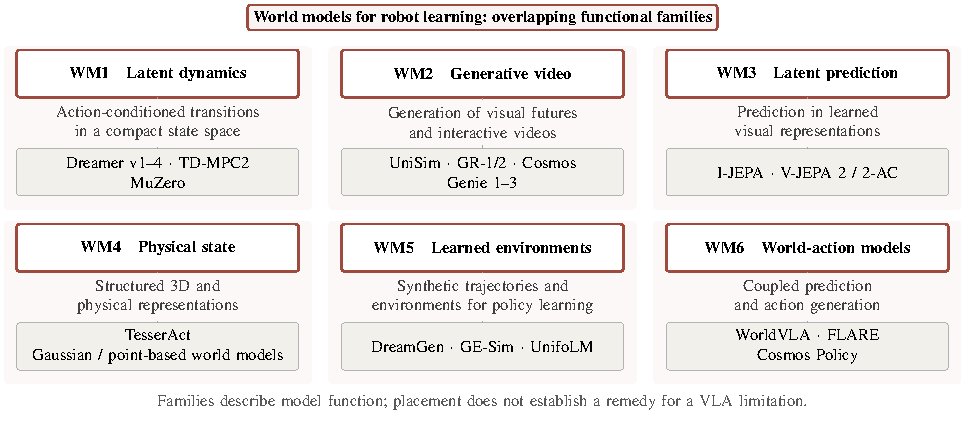
\includegraphics[width=0.95\linewidth]{figures/wm-taxonomy.pdf}
\caption{\textcolor[RGB]{104,48,148}{Functional taxonomy of predictive systems relevant to robot learning, including foundational and manipulation-oriented examples. Families overlap and do not by themselves establish that a system remedies a particular VLA limitation.}}
\label{fig:wm-taxonomy}
\end{figure*}


\subsection{WM3: Latent Prediction}
\label{sec:wm3}

Latent-predictive models avoid reconstructing pixels and instead forecast task-relevant representations. The goal is to retain useful dynamics while reducing the cost and uncertainty associated with detailed visual generation.

I-JEPA and V-JEPA established representation-space prediction for images and video~\cite{ijepa,vjepa}. V-JEPA~2 scales this objective through action-free video pretraining, while V-JEPA~2-AC introduces an action-conditioned predictor for robotic planning~\cite{vjepa2}. The adapted model outperforms Octo on two reported pick-and-place tasks without task-specific demonstrations. Its planning time is also substantially lower than that of the evaluated pixel-space baseline. However, the comparison uses different models and candidate counts, and the reported latency remains above typical control rates.

DINO-WM demonstrates that pretrained visual features can support planning without pixel reconstruction~\cite{dinowm}. LaWAM predicts latent visual subgoals for a VLA policy~\cite{lawam}, while VLA-JEPA integrates latent prediction more directly with action learning~\cite{jepavla}. These systems suggest that latent prediction may provide a better balance between foresight and inference cost. Evidence for the contribution of passive video remains indirect because current studies do not isolate it through controlled data ablations.

\subsection{WM4: Physical State Models}
\label{sec:wm4}

Pixel and latent representations may omit persistent geometry or contact state. Physical world models instead predict within representations that make three-dimensional structure and interaction more explicit.

TesserAct predicts multiple visual and geometric modalities to construct temporally consistent scenes~\cite{tesseract}. Gaussian World Models propagate dynamics through explicit Gaussian representations~\cite{gaussianworld}, while ManiGaussian applies dynamic splatting to manipulation~\cite{manigaussian}. PhysDreamer estimates material properties for physically grounded interaction~\cite{physdreamer}. Tactile world-action models extend prediction to contact-rich behavior~\cite{dreamtac,touchworld}.

This family addresses physical grounding more directly than appearance-based prediction. It may also provide state variables on which constraints can be imposed. However, comparative manipulation evidence remains limited. Explicit geometry improves the representation of the world, but it does not by itself guarantee accurate dynamics or safe control.

\subsection{WM5: Learned Environments}
\label{sec:wm5}

World models can also serve as environments in which data are generated, policies are evaluated, or reinforcement-learning agents are trained. These roles are attractive because physical interaction is expensive and difficult to scale.

As a data engine, DreamGen generates visual trajectories for new tasks and labels them through inverse dynamics~\cite{dreamgen}. Training with these trajectories improves policy performance on previously unsupported behaviors. MimicGen and DexMimicGen provide related precedents through simulator-based recombination of demonstrations~\cite{mimicgen,dexmimicgen}. DreamGen extends the idea by using a learned video model rather than a conventional simulator.

As an evaluator, an action-conditioned model can predict the outcomes of a candidate policy without deploying it on hardware~\cite{policyeval}. GE-Sim applies this idea within Genie Envisioner~\cite{genieenvisioner}. However, PolaRiS shows that generated evaluations may hallucinate interactions or rank policies differently from physical evaluation~\cite{polaris}. Learned simulation is therefore not automatically a valid evaluation instrument.

World-Gymnast provides direct evidence for training a policy inside a learned environment and transferring it to a real robot~\cite{sharma2026worldgymnast}. Its learned-world-model package outperforms a conventional simulator on three of four tasks but performs worse on the fourth (Fig.~\ref{fig:worldgymnast-transfer}). The experiment demonstrates feasibility while also showing why task-specific outcomes should not be hidden by a single average. \textcolor[RGB]{104,48,148}{The evidence scope is specified in Section~\ref{par:evidence-scope}.}

\begin{figure*}[!t]
\centering
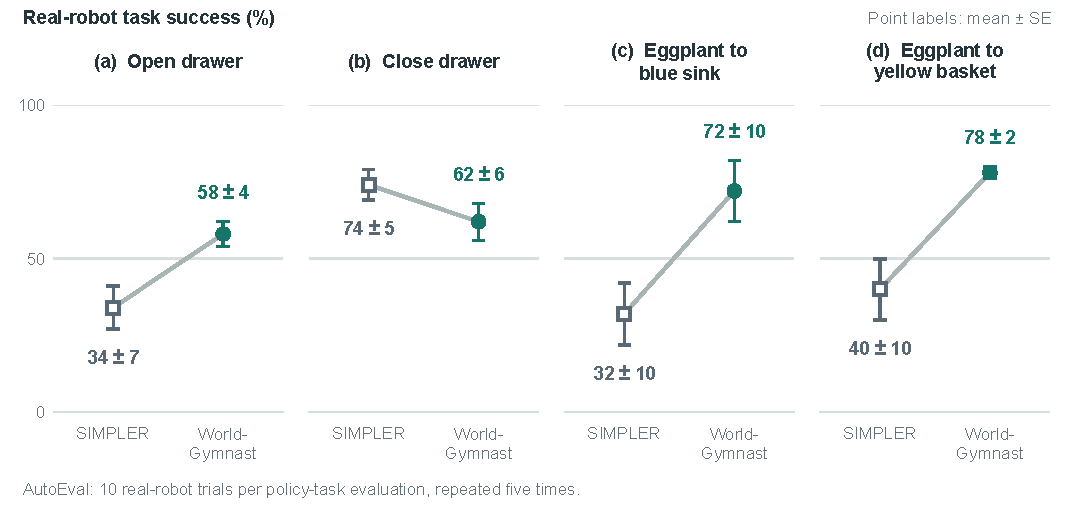
\includegraphics[width=0.97\linewidth]{figures/figure_09_task_slopes.pdf}
\caption{\textcolor[RGB]{104,48,148}{Task-level outcomes after reinforcement learning in SIMPLER and the World-Gymnast learned environment~\cite{sharma2026worldgymnast}. Squares and circles show source-reported means; vertical bars and numerical labels give the source-reported standard errors (SEs). Each policy--task evaluation used 10 real-robot trials and was repeated five times. All panels share a 0--100\% scale. Connecting segments join the two method-level means; they do not represent paired trial results or a training trajectory. The four-task package-level comparison does not isolate the effect of world-model quality.}}
\label{fig:worldgymnast-transfer}
\end{figure*}

\textcolor[RGB]{104,48,148}{The selected comparisons provide evidence for synthetic augmentation and bounded learned-practice implementations.} General policy evaluation and transferable imagined training remain unresolved.

\subsection{WM6: World-Action Models}
\label{sec:wm6}

World-action models combine predictive and control objectives within a shared architecture. This design can use prediction to improve the learned representation without requiring a separate planner during every action query. It can also expose future-state or value predictions when more deliberate decision making is needed.

\textcolor[RGB]{104,48,148}{Joint prediction and control predates WorldVLA. Seer combines future-state prediction with inverse dynamics, Video Prediction Policy supplies predictive visual representations to a policy, and Unified World Models couples video and action diffusion in a model that can be conditioned for policy, forward-dynamics, and inverse-dynamics roles~\cite{seer,vpp,uwm}. These approaches provide different interfaces between prediction and action. WorldVLA contributes an autoregressive formulation within this wider sequence of work; joint modeling should not be attributed to it as the first instance~\cite{worldvla}.}

WorldVLA jointly learns action generation and future-frame prediction~\cite{worldvla}. Its ablations show that predictive supervision can improve policy performance, although the gains depend on the action-decoding configuration. The study does not evaluate explicit rollout-based comparison among alternative actions. Auxiliary prediction and candidate-action search should therefore be treated as different mechanisms.

FLARE aligns policy representations with predicted future latents and supports training with action-free video~\cite{flarewm}. DreamVLA and tactile world-action systems extend joint prediction toward broader world knowledge and contact-rich interaction~\cite{dreamvla,dreamtac,touchworld}. StructVLA uses sparse structured foresight~\cite{structvla}, while LaWAM predicts latent subgoals to reduce inference cost~\cite{lawam}. These methods explore different positions on the trade-off between predictive detail and control latency.

\textcolor[RGB]{104,48,148}{Cosmos Policy adapts a video world model to predict actions, future states, and values~\cite{cosmospolicy}. It evaluates direct execution and a separate planning package; Section~\ref{par:evidence-scope} states the scope and attribution limits of the latter.}

Unified architectures show that prediction and action can reinforce one another within a shared model. They do not yet establish that every policy benefits from explicit planning or that predicted values provide calibrated safety information.

% Retain the existing limitation-to-mechanism figure here.
% Retain the existing architecture comparison figure here.

\subsection{Evidence Map}
\label{sec:evidence-map}
\textcolor[RGB]{104,48,148}{Table~\ref{tab:matrix} presents selected, source-linked comparisons for the six limitations. We use \emph{direct} when the reported comparison measures the stated outcome under a relevant intervention or reference evaluation, and \emph{indirect} when the argument relies on a different outcome, domain, or untested attribution. A direct comparison can evaluate a complete package without isolating each component. \emph{Prospective} denotes a proposed link without an outcome measurement in the cited example. Outcome direction is recorded separately as favorable, adverse, mixed, or inconclusive; adverse evidence can therefore be direct. These labels describe claims, not whole papers or a formal certainty grade.}

\textcolor[RGB]{104,48,148}{\noindent\textbf{Scope of the selected comparisons.}\label{par:evidence-scope}
WorldVLA's auxiliary-prediction comparisons concern policy success, and Cosmos Policy's refined planning comparison concerns completion on two ALOHA tasks; neither isolates L1 recovery. World-Gymnast's physical comparison covers four held-out tasks with mixed task-level outcomes and different training support across packages; its distractor and instruction extensions are evaluated within WorldGym. DreamGen tests neural-trajectory training for novel behaviors and environments without collecting task-specific teleoperation trajectories, but does not establish an interchangeable budget of video and robot hours~\cite{worldvla,cosmospolicy,sharma2026worldgymnast,dreamgen}.}

\textcolor[RGB]{104,48,148}{PolaRiS provides direct adverse evidence for the tested Ctrl-World evaluation pipeline by comparing its policy rankings with physical outcomes~\cite{polaris}. Physical grounding and consequence-aware safety require their own intervention and violation measurements; generic prediction or task-value accuracy is insufficient. The companion selected-example ledger records these distinctions. It is a revision-time audit of illustrative comparisons, not an exhaustive coding of the included-paper corpus or a prevalence estimate.}

\textcolor[RGB]{104,48,148}{Figure~\ref{fig:matrixfig} summarizes this bounded audit. Five of its six sources report physical-robot outcomes in a selected empirical comparison. WorldVLA contributes one matched auxiliary-prediction component ablation, whereas PolaRiS contributes one paired validation against physical policy rankings; these designs answer different questions and are counted separately. The filtered ledger, study identifiers, source versions and locators, and plotting script accompany the figure. Corpus-wide frequencies would require additional structured extraction.}

\subsection{Limitations of World Models}
\label{sec:wmweak}

World models introduce their own sources of error. Perceptual quality does not guarantee control-consistent dynamics. \textcolor[RGB]{104,48,148}{The generator-level association discussed in Section~\ref{sec:l4} cannot establish control validity~\cite{physicsiq}.} Long-horizon predictions can also drift as small model errors accumulate. \textcolor[RGB]{104,48,148}{Learned prediction introduces model error that can compound with policy, estimation, and execution errors.}

\textcolor[RGB]{104,48,148}{\noindent\textbf{Prediction and search cost.}\label{sec:deliberation-cost}
Inference time is a cost of a predictive mechanism, rather than a seventh VLA limitation. The V-JEPA~2 comparison reports approximately 16 seconds per selected action for its latent planner and four minutes for the Cosmos planning baseline on the same GPU, with different candidate counts and model configurations~\cite{vjepa2}. It measures those implementations rather than the isolated effect of prediction space. FLARE instead supervises future representations during policy training; this is distinct from online multi-candidate search~\cite{flarewm}. The additional cost therefore depends on how prediction enters the control loop.}

\textcolor[RGB]{104,48,148}{Reported rates must identify their operating level: actuator or action execution, policy/chunk inference, high-level reasoning, or complete planning latency. For example, $\pi_0$ reports high-rate action chunks, whereas Helix's vendor report distinguishes a 200-Hz reactive policy from a 7--9-Hz semantic system~\cite{pi0,helix}. These values should not be treated as interchangeable end-to-end planning rates. Evaluation should report the observation-to-command delay, chunk duration, hardware, asynchronous execution, and missed task-specific deadlines.}

Learned simulators also inherit biases from their training data. PolaRiS demonstrates that generated rollouts can hallucinate interactions and mis-rank policies~\cite{polaris}. Synthetic trajectories may pass related errors into the policy that learns from them. These risks become harder to assess when the model or evaluation system is closed, as in several vendor-reported platforms.

World models should therefore be judged by decision utility and transfer to physical control rather than by prediction quality alone. Current evidence does not support a general conclusion that predictive systems outperform direct policies across robotic manipulation.

\medskip
\noindent\textbf{Summary.}
World models now support latent planning, generative simulation, representation learning, physical-state prediction, imagined practice, and unified action generation. \textcolor[RGB]{104,48,148}{The selected manipulation comparisons document benefits from synthetic data and auxiliary predictive training.} Evidence for candidate comparison and real-world learned practice remains narrow. Physical validity, evaluation transfer, control-rate planning, and consequence-aware safety remain open. The following section examines these claims under their reported evaluation protocols.

% Retain Table~\ref{tab:matrix} and Table~\ref{tab:wm-master} here.

\begin{figure*}[!t]
\centering
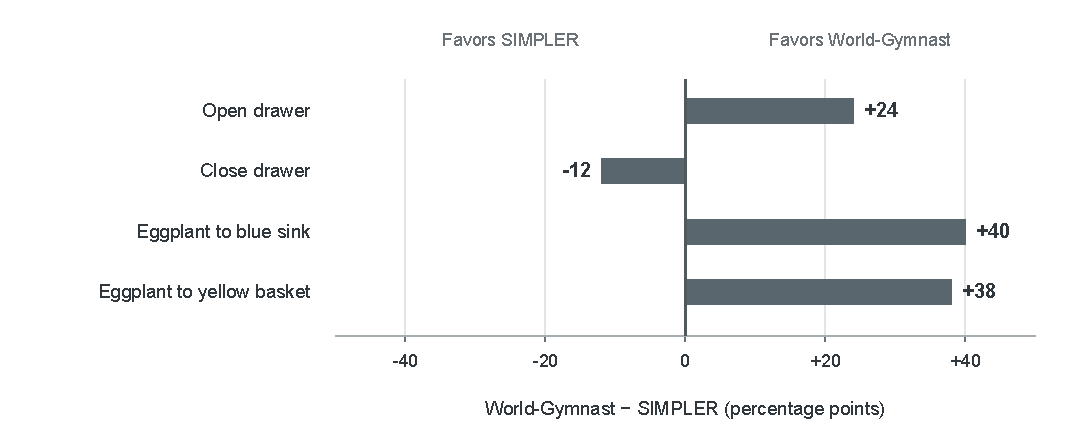
\includegraphics[width=0.97\linewidth]{figures/figure_10_task_differences.pdf}
\caption{\textcolor[RGB]{104,48,148}{Differences in the source-reported real-robot task-success means from Fig.~\ref{fig:worldgymnast-transfer}~\cite{sharma2026worldgymnast}. Each bar shows World-Gymnast minus SIMPLER in percentage points (pp); positive values favor World-Gymnast and negative values favor SIMPLER. The axis is symmetric about zero. These four descriptive differences use the same AutoEval experiment, not additional evaluations. Source-reported standard errors and the evaluation protocol are retained in Fig.~\ref{fig:worldgymnast-transfer}; no difference confidence interval or statistical significance is inferred.}}
\label{fig:worldgymnast-real}
\end{figure*}

\begin{figure*}[!tb]
\centering
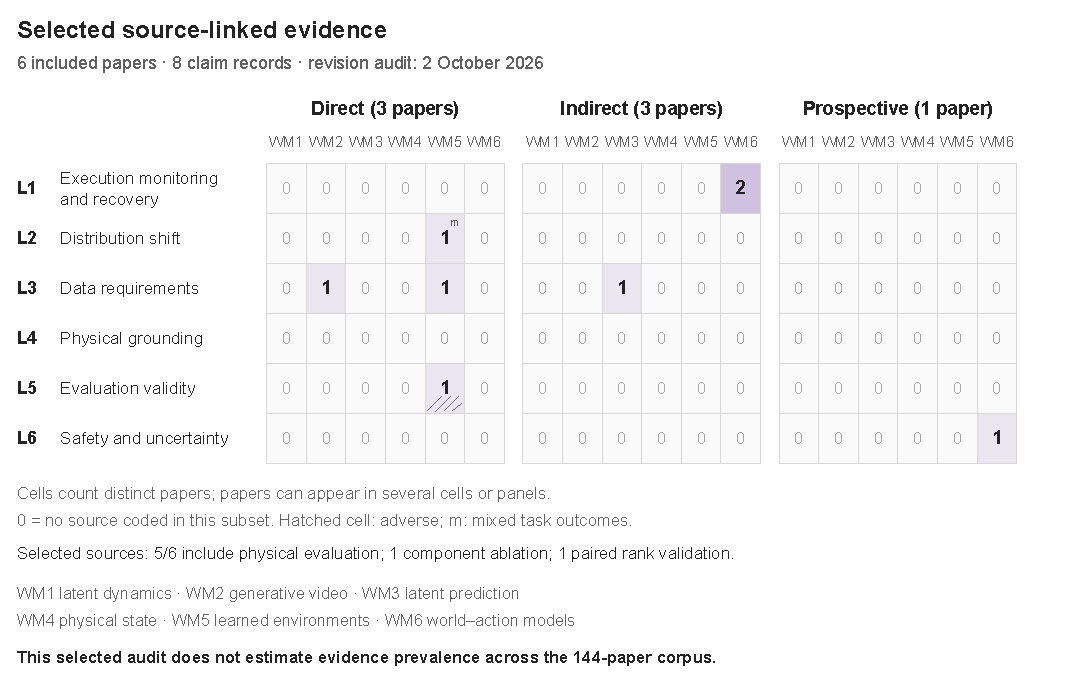
\includegraphics[width=0.99\linewidth]{figures/selected-evidence-heatmap.pdf}
\caption{\textcolor[RGB]{104,48,148}{Selected source-linked limitation--mechanism evidence from eight claim records covering six included papers~\cite{worldvla,cosmospolicy,sharma2026worldgymnast,dreamgen,vjepa2,polaris}. Cells count distinct papers; papers can occur in multiple cells or panels. Direct, indirect, and prospective describe correspondence to the stated outcome; hatching marks adverse evidence and $m$ marks mixed task outcomes. Zero denotes no coded source in this subset, not absence of evidence in the corpus. Deployment-cost rows, contextual generator benchmarks, and vendor-only sources are excluded. This audit does not estimate prevalence among the 144 included papers.}}
\label{fig:matrixfig}
\end{figure*}



\begin{figure*}[!tb]
\centering
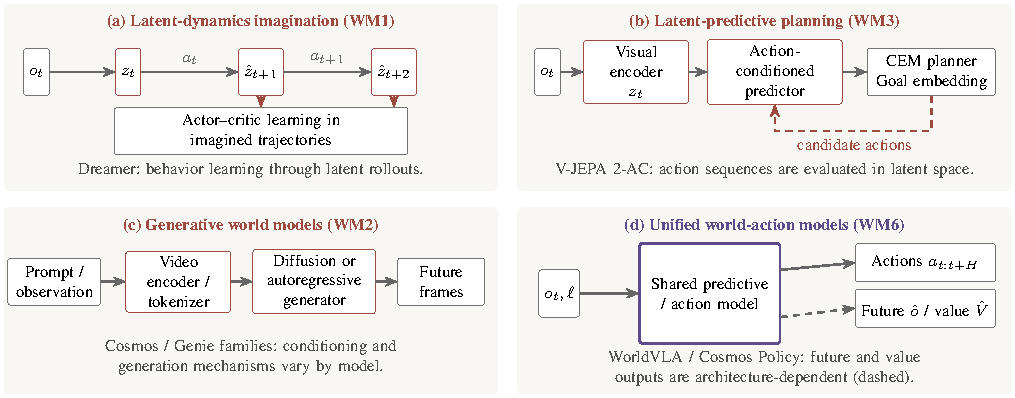
\includegraphics[width=0.99\linewidth]{figures/wm-architectures.pdf}
\caption{\textcolor[RGB]{104,48,148}{Schematic interfaces across world-model families: (a) latent-dynamics imagination for actor--critic learning (WM1), (b) action-conditioned latent prediction with cross-entropy-method planning (WM3), (c) visual-future generation with model-specific conditioning (WM2), and (d) coupled prediction and action generation (WM6). Dashed outputs in (d) depend on the architecture.}}
\label{fig:deepdives}
\end{figure*}
% -------------------------------------------------------------------------
% Table III — Limitation-to-candidate-mechanism matrix
% -------------------------------------------------------------------------
\begin{table*}[!t]
\caption{Limitation-to-candidate-mechanism matrix. The final column keeps
\emph{limitation evidence} separate from \emph{mechanism-effect evidence}.
\textcolor[RGB]{104,48,148}{Direct, indirect, and prospective describe the claim--evidence relationship; adverse describes outcome direction separately. These are not overall certainty grades or causal conclusions.}
Mechanisms remain candidates rather than established remedies
(Sec.~\ref{sec:wmweak}).}
\label{tab:matrix}
\centering
\scriptsize
\setlength{\tabcolsep}{4pt}
\begin{tabular}{p{3.0cm}p{3.2cm}p{3.2cm}p{5.6cm}}
\toprule
VLA limitation and its evidence & Candidate predictive mechanism (group) & Representative systems & Mechanism-effect evidence \\
\midrule
\textcolor[RGB]{104,48,148}{L1 Execution monitoring and recovery require controlled failure tests~\cite{pi0,recovla}} & \textcolor[RGB]{104,48,148}{Action-conditioned prediction and outcome monitoring (WM6)} & \textcolor[RGB]{104,48,148}{WorldVLA; Cosmos Policy} & \textcolor[RGB]{104,48,148}{\emph{Indirect for recovery.} Task-success or completion gains do not isolate error detection, recovery latency, or correction following an imposed failure~\cite{worldvla,cosmospolicy}.} \\
\addlinespace[2pt]
\textcolor[RGB]{104,48,148}{L2 Transfer can change across layouts, cameras, instructions, and embodiments~\cite{liberoplus}} & \textcolor[RGB]{104,48,148}{Learned practice environments (WM5)} & \textcolor[RGB]{104,48,148}{World-Gymnast} & \textcolor[RGB]{104,48,148}{\emph{Direct, package-level, mixed.} Physical held-out-task transfer is measured; distractor/instruction extensions are evaluated in WorldGym. Neither isolates one shift-handling component~\cite{sharma2026worldgymnast}.} \\
\addlinespace[2pt]
\textcolor[RGB]{104,48,148}{L3 Robot demonstrations require substantial collection effort~\cite{pi0,oxe}} & \textcolor[RGB]{104,48,148}{Synthetic trajectories and video pretraining (WM2, WM3, WM5)} & \textcolor[RGB]{104,48,148}{DreamGen; V-JEPA~2/2-AC} & \textcolor[RGB]{104,48,148}{\emph{Direct for the synthetic-data pipeline.} DreamGen Table~1 reports 11.2\% to 43.2\% on new behaviors and 0\% to 28.5\% on new environments~\cite{dreamgen}. These are task scores with partial credit, not robot-hours equivalence. Passive-video substitution remains \emph{indirect}~\cite{vjepa2}.} \\
\addlinespace[2pt]
\textcolor[RGB]{104,48,148}{L4 Physical grounding needs policy-level intervention tests; generator failures are contextual evidence~\cite{physicsiq,wmbench}} & \textcolor[RGB]{104,48,148}{Physical-state prediction and contact-aware representations (WM4)} & \textcolor[RGB]{104,48,148}{TesserAct; GWM} & \textcolor[RGB]{104,48,148}{\emph{Indirect/prospective.} The cited video benchmarks do not measure VLA control, and the selected comparisons do not isolate gains from mass, friction, or contact prediction~\cite{tesseract,gaussianworld}.} \\
\addlinespace[2pt]
\textcolor[RGB]{104,48,148}{L5 Learned evaluation must preserve physical policy rankings~\cite{polaris}} & \textcolor[RGB]{104,48,148}{Learned simulators and policy evaluators (WM5)} & \textcolor[RGB]{104,48,148}{Ctrl-World~\cite{ctrlworld}; GE-Sim; WorldEval} & \textcolor[RGB]{104,48,148}{\emph{Direct, adverse.} PolaRiS compares the tested Ctrl-World evaluation pipeline with physical outcomes and identifies hallucinated interactions and policy mis-ranking~\cite{polaris}. This finding concerns that pipeline.} \\
\addlinespace[2pt]
\textcolor[RGB]{104,48,148}{L6 Safety requires calibrated risk, enforcement, and fallback evaluation~\cite{knowno,safelibero,gemini15}} & \textcolor[RGB]{104,48,148}{Consequence and uncertainty estimates with runtime protection (WM6; prospective WM4)} & \textcolor[RGB]{104,48,148}{Cosmos Policy; safety benchmarks} & \textcolor[RGB]{104,48,148}{\emph{Prospective.} Task-value prediction does not establish calibrated violation risk or irreversibility estimates; dedicated safety outcomes are needed~\cite{cosmospolicy}.} \\
\bottomrule
\end{tabular}
\end{table*}

% -------------------------------------------------------------------------
% Table IV — Representative world models by group
% -------------------------------------------------------------------------
\begin{table*}[!t]
\caption{Representative world models and predictive systems by overlapping
taxonomy group. Year denotes the first public report. State: Pix = pixel/video,
Lat = latent, 3D = geometry. A-cond: \cmark~= executable-action conditioning,
L = learned latent actions, J = joint future video/action generation,
(\cmark)~= game/interface controls; --- = no such conditioning.
Int: the prediction module is queried during closed-loop control, learned
simulation, or evaluation; this does not by itself imply candidate-action planning.
\textcolor[RGB]{104,48,148}{An Int dash indicates that predictive outputs are not used in the listed deployment mode; it does not deny a model's other prediction capabilities.}
Open: \cmark~= verified official public code or weights; --- = no verified release.
Task-conditioned prediction and auxiliary pretraining are distinguished from
action-conditioned transitions. Results use each source's own protocol.}
\label{tab:wm-master}
\centering
\scriptsize
\setlength{\tabcolsep}{3.5pt}
\begin{tabular}{p{2.7cm}p{1.35cm}p{0.9cm}p{1.2cm}cccp{5.9cm}}
\toprule
Model & Year & Grp & State & A-cond & Int & Open & Headline result (own protocol) \\
\midrule
World Models~\cite{worldmodels2018} & 2018 & WM1 & Lat & (\cmark) & \cmark & \cmark & Policy learning in imagined CarRacing/Doom environments \\
PlaNet~\cite{planet} & 2018 & WM1 & Lat & \cmark & \cmark & \cmark & Latent MPC from pixels \\
DreamerV3~\cite{dreamerv3} & 2023 & WM1 & Lat & \cmark & \cmark & \cmark & 150+ tasks, one configuration; Nature publication in 2025 \\
TD-MPC2~\cite{tdmpc2} & 2023 & WM1 & Lat & \cmark & \cmark & \cmark & 80/104 tasks, single 317M agent \\
Dreamer 4~\cite{dreamer4} & 2025 & WM1 & Lat & (\cmark) & \cmark & --- & Offline imagined-policy training; Minecraft diamond acquisition \\
UniPi~\cite{unipi} & 2023 & WM2 & Pix & --- & --- & --- & Text-conditioned video plus inverse dynamics \\
UniSim~\cite{unisim} & 2023 & WM2 & Pix & \cmark & \cmark & --- & Interactive learned simulator \\
GR-1~\cite{gr1} & 2023 & WM2 & Pix & --- & --- & \cmark & CALVIN ABCD$\to$D: 94.9\% first-task success; 4.21 chain length \\
Cosmos~\cite{cosmos} & 2025 & WM2 & Pix & --- & --- & \cmark & Open WFM platform, 2048$\times$ tokenizer \\
Genie 3~\cite{genie3} & 2025 & WM2 & Pix & (\cmark) & \cmark & --- & Real-time 720p worlds, minutes \\
Genie Envisioner~\cite{genieenvisioner} & 2025 & WM2/5 & Pix & \cmark & \cmark & \cmark & GE-Act solves tasks where VLAs: 0\% \\
V-JEPA 2~\cite{vjepa2} & 2025 & WM3 & Lat & --- & --- & \cmark & Action-free video representation pretraining \\
V-JEPA 2-AC~\cite{vjepa2} & 2025 & WM3 & Lat & \cmark & \cmark & \cmark & Image-goal Franka planning; 16 s/query; 10 trials/skill/config. \\
VLA-JEPA~\cite{jepavla} & 2026 & WM3/6 & Lat & L & --- & \cmark & Latent-action predictive pretraining for robot policies \\
LaWAM~\cite{lawam} & 2026 & WM3/6 & Lat & L & \cmark & \cmark & Predicted latent subgoals; LIBERO 98.6\%; 187 ms/chunk \\
TesserAct~\cite{tesseract} & 2025 & WM4 & 3D & --- & --- & \cmark & Text-conditioned RGB-D-normal futures and inverse dynamics \\
GWM~\cite{gaussianworld} & 2025 & WM4/5 & 3D & \cmark & \cmark & \cmark & Gaussian-state neural simulation for model-based policy optimization \\
DreamGen~\cite{dreamgen} & 2025 & WM5 & Pix & --- & --- & \cmark & Synthetic video plus inverse-dynamics labels \\
GE-Sim~\cite{genieenvisioner} & 2025 & WM5 & Pix & \cmark & \cmark & \cmark & Closed-loop neural simulator \\
WorldEval~\cite{policyeval} & 2025 & WM5 & Pix & \cmark & \cmark & \cmark & Hardware-free policy ranking \\
UnifoLM-WMA-0~\cite{unifolm} & 2025 & WM5 & Pix & \cmark & \cmark & \cmark & Open humanoid WM stack (no quant.) \\
World-Gymnast~\cite{sharma2026worldgymnast} & 2026 & WM5 & Pix & \cmark & \cmark & \cmark & Four-task real-robot transfer: three positive and one adverse simulator comparison \\
DreamDojo~\cite{dreamdojo} & 2026 & WM2/5 & Pix & \cmark & \cmark & \cmark & 44k h human-video pretraining; robot-action simulation, evaluation and planning \\
\textcolor[RGB]{104,48,148}{Unified World Models~\cite{uwm}} & \textcolor[RGB]{104,48,148}{2025} & \textcolor[RGB]{104,48,148}{WM6} & \textcolor[RGB]{104,48,148}{Lat+act} & \textcolor[RGB]{104,48,148}{J} & \textcolor[RGB]{104,48,148}{---} & \textcolor[RGB]{104,48,148}{\cmark} & \textcolor[RGB]{104,48,148}{Coupled video/action diffusion; policy, forward- and inverse-dynamics modes} \\
WorldVLA~\cite{worldvla} & 2025 & WM6 & Pix+act & \cmark & --- & \cmark & Auxiliary action-conditioned prediction improves LIBERO policy ablations \\
FLARE~\cite{flarewm} & 2025 & WM6 & Lat & \cmark & --- & \cmark & Up to +26\%; action-free co-training \\
DreamVLA~\cite{dreamvla} & 2025 & WM6 & Pix+lat & --- & \cmark & \cmark & Predicted dynamics/depth/semantics condition action diffusion \\
Cosmos Policy~\cite{cosmospolicy} & 2026 & WM6 & Pix+act & \cmark & \cmark & \cmark & Direct policy: LIBERO 98.5\%; rollout-refinement + best-of-8: +12.5 points on two ALOHA tasks \\
DreamZero~\cite{dreamzero} & 2026 & WM6 & Pix+act & J & \cmark & \cmark & 14B joint video--action model; Flash: $\sim$7 Hz chunk inference (2 GB200s) \\
StructVLA~\cite{structvla} & 2026 & WM6 & Pix+act & --- & --- & \cmark & Sparse visual planning pretraining followed by action-policy tuning \\
HarmoWAM~\cite{harmowam} & 2026 & WM6 & Pix+act & --- & \cmark & \cmark & Video foresight with adaptive transit/manipulation action experts \\
\bottomrule
\end{tabular}
\end{table*}






\section{Evaluation Evidence}
\label{sec:benchmarks}

Evaluation remains fragmented across VLA policies and world models. Policy benchmarks primarily measure task completion, generalization, and robustness, whereas world-model benchmarks emphasize perceptual quality, physical consistency, or predictive accuracy. Few protocols evaluate whether prediction improves manipulation decisions. This separation limits cross-family comparison and creates a central measurement gap: prediction quality, decision utility, and control performance are related but not interchangeable.

\subsection{Benchmark Scope}

VLA evaluation spans simulated manipulation, matched simulation and physical platforms, and distributed real-robot testing. LIBERO is widely used for language-conditioned tabletop manipulation~\cite{liu2023libero}, while LIBERO-Plus evaluates robustness under changes in viewpoint, layout, language, and other environmental factors~\cite{liberoplus}. CALVIN emphasizes long-horizon task sequences and generalization across environments~\cite{calvin}. RLBench, ManiSkill, RoboCasa, Meta-World, and VLABench extend coverage across multi-task manipulation, procedurally generated scenes, and language-conditioned reasoning~\cite{rlbench,maniskill3,robocasa,metaworld,vlabench}.

Other benchmarks target particular evaluation gaps. SimplerEnv constructs control-matched simulations of two physical robot platforms~\cite{simplerenv}. THE COLOSSEUM applies systematic perturbations to evaluate generalization~\cite{colosseum}, while FurnitureBench and BEHAVIOR-1K broaden evaluation toward assembly and household activity~\cite{furniturebench,behavior1k}. RoboArena supports distributed real-robot comparison through A/B evaluation~\cite{roboarena}. Large datasets such as Open X-Embodiment, DROID, BridgeData~V2, AgiBot World, RH20T, and RoboMIND also provide held-out evaluation splits, although they are training corpora rather than controlled benchmarks~\cite{oxe,droid,bridgedata,agibotworld,rh20t,robomind}.

World-model evaluation uses a different set of criteria. WorldModelBench assesses instruction-conditioned generation against physical principles~\cite{wmbench}, Physics-IQ isolates physical understanding using paired real videos~\cite{physicsiq}, and VBench-2.0 evaluates intrinsic faithfulness in generated video~\cite{vbench2}. EWMBench focuses more directly on embodied prediction~\cite{genieenvisioner}. WorldArena extends evaluation from perceptual quality to functional roles, including synthetic-data generation, policy evaluation, and action planning~\cite{worldarena}. WorldArena~2.0 adds visuotactile observations, interactive reinforcement-learning environments, and simulated and physical platforms across multiple embodiments~\cite{shang2026worldarena2}.

\textcolor[RGB]{104,48,148}{Recent benchmarks seek to connect the two evaluation traditions.} ManipArena evaluates VLA and world-model approaches under a shared real-world protocol with synchronized real-to-simulation environments~\cite{maniparena}. WorldArena and WorldArena~2.0 assess world models according to their functional contribution to learning and control~\cite{worldarena,shang2026worldarena2}. These benchmarks narrow the divide, but they remain recent and have not yet established a common evaluation standard.

The underlying issue is that four distinct notions of world-model quality are often conflated. A model may produce realistic videos without preserving physical dynamics or ranking candidate actions correctly. Conversely, an abstract latent model may support effective decisions without generating visually realistic observations. Table~\ref{tab:fournotions} separates these notions.

\begin{table}[!t]
\caption{Distinct notions of world-model quality. Each requires a different evaluation instrument, and strong performance on one dimension does not imply strong performance on another.}
\label{tab:fournotions}
\centering
\scriptsize
\setlength{\tabcolsep}{3pt}
\begin{tabular}{p{1.5cm}p{2.8cm}p{2.9cm}}
\toprule
Notion & What it measures & Evidence of decoupling \\
\midrule
Visual fidelity &
Perceptual realism of generated rollouts &
An eight-model comparison found a negative but nonsignificant association between MLLM-based visual judgments and physical understanding ($r=-0.46$, $p=.249$); FVD was not examined~\cite{physicsiq} \\
\addlinespace[2pt]

Physical fidelity &
Consistency with geometry, contact, and mechanics &
Physically inconsistent events can occur in visually plausible generations~\cite{wmbench} \\
\addlinespace[2pt]

Decision utility &
Whether predictions rank candidate actions or policies correctly &
Latent models can support planning without generating pixels~\cite{vjepa2}; WorldArena identifies a perception--functionality gap across 14 world models~\cite{worldarena} \\
\addlinespace[2pt]

Control performance &
Task success when the model is coupled to a controller &
Prediction quality does not necessarily transfer to manipulation success; gains have been demonstrated only for particular joint prediction--action systems~\cite{worldvla,cosmospolicy} \\
\bottomrule
\end{tabular}
\end{table}

Table~\ref{tab:benchmarks} summarizes the resulting evaluation landscape. Its purpose is to identify complementary coverage and unresolved gaps, not to imply that results obtained under different protocols are directly comparable.

\begin{table*}[!t]
\caption{Benchmark landscape for VLA policies and world models. Type: S = simulation, R = real, and S/R = matched simulation and physical evaluation. Horizon: S = single-stage and L = multi-stage.}
\label{tab:benchmarks}
\centering
\scriptsize
\setlength{\tabcolsep}{3pt}
\begin{tabular}{p{3.7cm}llp{0.8cm}p{4.4cm}p{4.0cm}}
\toprule
Benchmark & Year & Type & Hor. & Primary focus & Principal caveat \\
\midrule
\multicolumn{6}{l}{\emph{VLA and policy benchmarks}} \\
LIBERO~\cite{liu2023libero} & 2023 & S & S/L &
130 language-conditioned tasks in four suites &
High reported scores; sensitivity to perturbations~\cite{liberoplus} \\

LIBERO-Plus~\cite{liberoplus} & 2025 & S & S/L &
Robustness across seven perturbation axes &
Restricted to the scope of the underlying LIBERO tasks \\

SimplerEnv~\cite{simplerenv} & 2024 & S/R & S &
Control-matched simulation of two physical platforms &
Limited embodiment coverage \\

CALVIN~\cite{calvin} & 2022 & S & L &
Long-horizon sequences and ABC$\to$D generalization &
Single simulated robot platform \\

RLBench~\cite{rlbench} & 2020 & S & S/L &
One hundred manipulation tasks &
Dependence on scripted demonstrations \\

ManiSkill3~\cite{maniskill3} & 2024 & S & S/L &
GPU-parallel large-scale evaluation &
Simulation-only physics \\

RoboCasa~\cite{robocasa} & 2024 & S & L &
Generated kitchen environments &
Simulation and layout bias \\

Meta-World~\cite{metaworld} & 2019 & S & S &
Multi-task and meta-reinforcement learning &
Limited visual diversity and saturation on some tasks \\

RoboArena~\cite{roboarena} & 2025 & R & S/L &
Distributed real-robot A/B evaluation &
Throughput and variation across sites \\

OXE, DROID, BridgeData~V2, and AgiBot World~\cite{oxe,droid,bridgedata,agibotworld} &
2023--25 & R & --- &
Training datasets with held-out evaluation splits &
Not controlled benchmarks \\
\midrule
\multicolumn{6}{l}{\emph{World-model benchmarks}} \\
WorldModelBench~\cite{wmbench} & 2025 & S/R & S &
Instruction-conditioned generation and physical consistency &
Evaluates generation rather than control \\

Physics-IQ~\cite{physicsiq} & 2025 & R & S &
Physical understanding from paired videos &
No action conditioning \\

VBench-2.0~\cite{vbench2} & 2025 & S/R & S &
Intrinsic faithfulness, including physical behavior &
Targets general video rather than robotics \\

EWMBench~\cite{genieenvisioner} & 2025 & S/R & S/L &
Scene, motion, and semantic quality in embodied prediction &
Closely associated with one system family \\

WorldArena~\cite{worldarena} & 2026 & S/R & S/L &
Perceptual and functional evaluation &
Recent benchmark with a limited task source \\

WorldArena~2.0~\cite{shang2026worldarena2} & 2026 & S/R & S/L &
Visuotactile prediction, interactive learning, and multi-embodiment evaluation &
Recent preprint without broad independent replication \\

ManipArena~\cite{maniparena} & 2026 & S/R & S/L &
Shared evaluation of VLAs and world models using real-to-simulation twins &
Recent benchmark restricted to 20 tasks \\
\bottomrule
\end{tabular}
\end{table*}

\subsection{Comparison Principles}
\label{sec:comparison-principles}

The available results support descriptive synthesis rather than statistical meta-analysis. Evaluations differ in embodiment, control frequency, observation inputs, training data, task splits, and reporting practice. \textcolor[RGB]{104,48,148}{Common effect measures and episode-level uncertainty are not consistently available in the selected comparisons.} Pooling their headline scores would therefore produce a precision that the underlying evidence does not support.

Results are compared only when their experimental conditions can be established. Scores obtained from different benchmarks are not used to rank systems. When configurations differ within the same benchmark, they are reported separately. This distinction is important for LIBERO, where camera inputs, proprioception, data filtering, training procedures, and suite coverage vary across studies. A shared benchmark name consequently does not imply a matched protocol.

\textcolor[RGB]{104,48,148}{Findings and limitations are interpreted in the context of each study's methods and evaluation protocols.} No confidence intervals or significance tests are inferred when the original study does not report the information required to calculate them.

\subsection{Shared-Benchmark Results}

Table~\ref{tab:libero} presents reported LIBERO results under their respective configurations. The scores illustrate progress within the benchmark family, but they should not be interpreted as a unified leaderboard.

The OpenVLA baseline reports a four-suite average of 76.5\%~\cite{openvla}. OpenVLA-OFT reports substantially higher performance after changing the training data, decoding method, and observation configuration~\cite{openvlaoft}. Its 95.3\% and 97.1\% averages correspond to different visual and proprioceptive inputs and must therefore remain separate. The $\pi_0$ result reported in the same study uses the modified data configuration and reaches 94.2\%~\cite{openvlaoft}.

SimpleVLA-RL evaluates reinforcement-learning post-training only on LIBERO-Long. Its 91.7\% one-demonstration result and 98.5\% full-trajectory result are informative within those settings but cannot be compared directly with four-suite averages~\cite{simplevlarl}. Cosmos Policy reports a 98.5\% four-suite average in direct-policy mode under its own filtered-data and observation configuration~\cite{cosmospolicy}. Establishing superiority among these systems would require matched training data, observations, task episodes, and statistical reporting.

\begin{table*}[!t]
\caption{Reported LIBERO success rates (\%) under protocol-specific configurations. Rows do not constitute a common leaderboard. Third denotes the third-person camera; wrist and proprio denote wrist imagery and proprioception. Dashes indicate unreported or inapplicable values.}
\label{tab:libero}
\centering
\scriptsize
\setlength{\tabcolsep}{3pt}
\begin{tabular}{p{3.0cm}p{5.0cm}ccccc}
\toprule
Model & Reported configuration & Spatial & Object & Goal & Long & Avg \\
\midrule
OpenVLA~\cite{openvla} &
Published baseline &
84.7 & 88.4 & 79.2 & 53.7 & 76.5 \\

OpenVLA-OFT~\cite{openvlaoft} &
Filtered training set; third-person image and language &
96.2 & 98.3 & 96.2 & 90.7 & 95.3 \\

OpenVLA-OFT~\cite{openvlaoft} &
Filtered training set; third-person and wrist images, optional proprioception, and language &
97.6 & 98.4 & 97.9 & 94.5 & 97.1 \\

$\pi_0$~\cite{openvlaoft} &
Result reported by the OFT study using its modified training and observation configuration &
96.8 & 98.8 & 95.8 & 85.2 & 94.2 \\

SimpleVLA-RL~\cite{simplevlarl} &
One demonstration per task; post-reinforcement-learning result &
--- & --- & --- & 91.7 & --- \\

SimpleVLA-RL~\cite{simplevlarl} &
Full-trajectory supervised and reinforcement-learning configuration &
--- & --- & --- & 98.5 & --- \\

Cosmos Policy~\cite{cosmospolicy} &
Direct parallel decoding; filtered policy data and unfiltered world/value training data &
98.1 & 100.0 & 98.2 & 97.6 & 98.5 \\
\bottomrule
\end{tabular}
\end{table*}

Evidence from other benchmarks is less complete. On SimplerEnv, discrete-diffusion decoding reports 71.2\% visual-matching performance for the Google Robot setting and 49.3\% overall performance for the Bridge setting~\cite{ddvla}. Memory-augmented policies report results at a similar level, although unresolved protocol details prevent a definitive comparison~\cite{memoryvla}. On the CALVIN ABC$\to$D split, GR-1 reports an increase from 88.9\% to 94.9\% after video-generative pretraining~\cite{gr1}. These findings suggest benefits within their respective settings, but they do not support cross-benchmark ranking.

\subsection{Cross-Family Profiles}

Table~\ref{tab:verdicts} summarizes representative evidence from the VLA and world-model families. The profiles illustrate different forms of contribution, including benchmark performance, real-world deployment, openness, efficiency, and functional prediction. Because these criteria are not measured on a common scale, the table is an evidence map rather than a ranking.

\begin{table*}[!t]
\caption{Representative evidence profiles across VLA and world-model families. Selection criteria differ across rows; the table therefore supports orientation rather than ranking.}
\label{tab:verdicts}
\centering
\scriptsize
\setlength{\tabcolsep}{3.5pt}
\begin{tabular}{p{2.4cm}p{3.0cm}p{2.2cm}p{7.7cm}}
\toprule
Group & Representative evidence & Related system & Basis and scope \\
\midrule
A Action tokens &
\textcolor[RGB]{104,48,148}{OpenVLA / FAST} &
SpatialVLA &
\textcolor[RGB]{104,48,148}{Autoregressive action tokens and frequency-space tokenization; deployment properties depend on the tokenizer and decoding configuration~\cite{openvla,fast}} \\

B Continuous actions &
\textcolor[RGB]{104,48,148}{OpenVLA-OFT / $\pi_{0.5}$} &
$\pi_0$ / GR00T N1 &
Open weights and deployment in previously unseen homes~\cite{pi05}; GR-2 reports 97.7\% under a gated, vendor-reported setting~\cite{gr2} \\

C Hierarchical reasoning &
Hi Robot / ECoT &
OneTwoVLA &
Open evidence for hierarchical execution and intermediate reasoning; Gemini Robotics 1.5 remains vendor-reported~\cite{gemini15} \\

D Spatial grounding &
SpatialVLA &
GraspVLA &
Source-traced gains from spatial action tokens; GraspVLA addresses the narrower grasping problem~\cite{spatialvla} \\

E Interactive learning &
SimpleVLA-RL &
RIPT-VLA &
LIBERO-Long improvement from 17.3\% to 91.7\% in the one-demonstration setting; a separate full-trajectory configuration reaches 98.5\%~\cite{simplevlarl} \\

F Efficient deployment &
SmolVLA &
BitVLA &
Competitive performance with consumer-GPU training and reduced computational requirements~\cite{smolvla} \\

G Embodiment &
$\pi_{0.5}$ &
GR00T N1.5 &
Open evidence for long-duration mobile manipulation~\cite{pi05}; Helix remains vendor-reported \\

\midrule
WM1 Latent dynamics &
Dreamer 4 &
TD-MPC2 &
Offline imagined learning in Minecraft~\cite{dreamer4}; broad latent-control evidence from TD-MPC2~\cite{tdmpc2} \\

WM2 Generative video &
Cosmos &
Genie Envisioner &
Open platform with source-traced licensing and technical documentation~\cite{cosmos}; Genie~3 interactivity remains vendor-reported~\cite{genie3} \\

WM3 Latent prediction &
V-JEPA 2-AC &
DINO-WM &
Image-goal Franka planning without task-specific demonstrations; evaluation uses ten trials per skill and configuration~\cite{vjepa2} \\

WM4 Physical state &
No comparable profile &
TesserAct / GWM &
Relevant systems exist, but no matched control comparison was identified \\

WM5 Learned environments &
DreamGen &
GE-Sim &
Quantified gains from generated training trajectories~\cite{dreamgen}; evidence for broader learned simulation remains limited \\

WM6 World-action models &
Cosmos Policy &
WorldVLA &
Direct-policy LIBERO average of 98.5\% and RoboCasa result of 67.1\%; a separate computationally intensive planning package improves two ALOHA tasks by 12.5 points~\cite{cosmospolicy}. WorldVLA reports gains from auxiliary predictive training~\cite{worldvla} \\
\bottomrule
\end{tabular}
\end{table*}

\textcolor[RGB]{104,48,148}{The profiles separate task-success measurements from tests of the predictive mechanism. A reported policy gain or prediction score does not by itself isolate how prediction contributes to physical manipulation.} \textcolor[RGB]{104,48,148}{The selected cross-family examples document auxiliary predictive training and synthetic trajectory generation.} Evidence for candidate-action comparison, policy evaluation inside learned environments, and real-time predictive control remains narrow.

\subsection{Interpretation}

The evidence cannot be reduced to a single system score. Task success, robustness, physical deployment, computational cost, data requirements, openness, and independent replication answer different questions. They are also measured on incompatible scales and have application-dependent importance. Assigning review-derived weights would therefore create an artificial ranking unsupported by the available studies.

For practical selection, systems should first be screened against non-negotiable constraints such as safety, hardware availability, control latency, and access. The remaining candidates can then be compared dimension by dimension under matched evaluation conditions. For research evaluation, the more important requirement is a protocol that measures prediction quality and manipulation performance within the same experiment.

The principal finding is therefore methodological as well as technical. \textcolor[RGB]{104,48,148}{A task-completion score or a plausible generated future does not, by itself, establish whether prediction supports a better decision.} Progress at the intersection of VLAs and world models requires joint evaluation of physical validity, uncertainty calibration, candidate ranking, control latency, and real-robot success.




\section{Research Directions}
\label{sec:roadmap}

The evidence synthesized in Table~\ref{tab:matrix} and Section~\ref{sec:benchmarks} identifies ten research directions for integrating predictive models with robotic control. These directions span model architecture, training data, evaluation, deployment, and safety. They are connected rather than independent: reliable deployment depends on predictive models that remain stable under interaction, evaluation protocols that measure decision utility, and assurance mechanisms that detect unsupported or unsafe predictions. \textcolor[RGB]{104,48,148}{Fig.~\ref{fig:roadmap} groups these directions thematically; it does not assign readiness levels, dependency arrows, or completion dates.}

\begin{figure*}[!t]
\centering
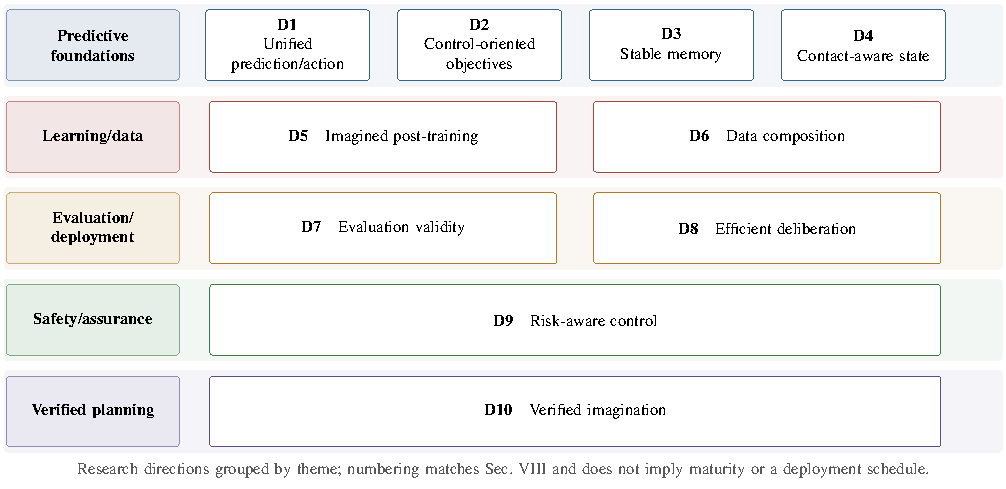
\includegraphics[width=0.95\linewidth]{figures/roadmap.pdf}
\caption{Illustrative dependency and readiness roadmap. The ten directions
of Sec.~\ref{sec:roadmap} (D1--D10) are arranged in five layers; arrows mark
dependencies, not dates. D10 asks when learned rollouts can be used inside a
formally specified runtime assurance and task-and-motion planning stack.}
\label{fig:roadmap}
\end{figure*}


\subsection{Predictive Foundations}

Four directions concern the predictive substrate itself: unified prediction and action, control-oriented objectives, long-horizon memory, and physically grounded state representations.

\noindent\textbf{D1: Unified prediction and action.}
World-action models increasingly use a shared architecture to predict environmental change and generate robot actions. Existing systems represent this integration through shared token vocabularies~\cite{worldvla}, alignment with future latent states~\cite{flarewm}, or adaptation of a pretrained world foundation model into a policy~\cite{cosmospolicy}. However, the conditions under which predictive supervision improves control remain unclear. Joint training may produce transferable representations, but it may also introduce competition for model capacity or optimization interference between prediction and action objectives.

Future work should isolate these effects through matched ablations of direct policies, auxiliary prediction, and explicit rollout-based planning. Important questions include how capacity should be distributed among prediction, action, and value heads; whether joint objectives obey identifiable scaling relationships; and when general world-foundation backbones such as Cosmos~\cite{cosmos} complement or replace purpose-built VLA architectures.

\noindent\textbf{D2: Control-oriented objectives.}
Perceptual realism is an incomplete objective for predictive control. Physics-IQ reports a negative but statistically nonsignificant association between its MLLM-based realism judgment and physical-understanding score across eight models ($r=-0.46$, $p=.249$)~\cite{physicsiq}. This result neither establishes independence between the two measures nor evaluates FVD, but it illustrates why appearance alone cannot establish decision utility.

A control-oriented model must respond correctly to changes in the applied action and preserve distinctions that affect task outcomes. Training objectives should therefore measure action sensitivity, state-transition consistency, candidate ranking, and closed-loop utility. EWMBench, WorldArena, and WorldArena~2.0 provide foundations for this direction by extending evaluation toward functional prediction, visuotactile interaction, and reinforcement-learning environments~\cite{genieenvisioner,worldarena,shang2026worldarena2}. The remaining challenge is to develop differentiable control-consistency objectives that can be applied during training and shown to improve physical manipulation.

\noindent\textbf{D3: Stable memory.}
Long-horizon prediction remains vulnerable to accumulated model error and loss of persistent state. Interactive consistency has been demonstrated for only limited durations, and some of the strongest claims remain vendor-reported~\cite{genie3}. Manipulation adds further difficulty because relevant objects may be occluded and contact state may not be recoverable from a single image.

Predictive systems therefore require memory that preserves object identity, geometry, task progress, and contact history across extended execution. Promising directions include retrieval-augmented prediction, explicit object-centric memory, and recurrent latent states with calibrated drift estimates. The gains reported for memory-augmented policies suggest that persistent context can already improve action generation~\cite{memoryvla}; equivalent evidence is still needed for world models. Evaluation should report prediction error as a function of rollout horizon and identify the horizon beyond which the model no longer supports reliable decisions.

\noindent\textbf{D4: Contact-aware state.}
Physical interaction cannot be represented adequately through visual appearance alone. Force- and tactile-conditioned policies show that contact modalities provide useful control information~\cite{forcevla,tactilevla}, while tactile world-action models extend predictive learning into contact-rich settings~\cite{dreamtac}. \textcolor[RGB]{104,48,148}{The selected evidence map does not establish a matched physical-property intervention result for these approaches.}

\textcolor[RGB]{104,48,148}{One promising direction represents force, compliance, friction, deformation, and contact mode explicitly and compares this choice with latent alternatives under controlled physical interventions.} Hybrid neural--analytic dynamics and differentiable contact models may combine the adaptability of learned prediction with stronger physical structure. Corresponding benchmarks should include tasks whose success depends on predicting forces or material responses, so that appearance-based shortcuts cannot produce high scores.

\subsection{Learning and Data}

The next two directions concern the use of learned environments for policy improvement and the composition of the data used to train them.

\noindent\textbf{D5: Imagined post-training.}
Reinforcement-learning improvements in VLA policies and advances in learned simulation suggest a common training loop: use a world model to generate interaction experience, optimize the policy within that environment, and validate the resulting behavior on the physical robot. \textcolor[RGB]{104,48,148}{World-Gymnast demonstrates physical transfer under the bounded comparison described in Section~\ref{par:evidence-scope}~\cite{sharma2026worldgymnast}.} Dreamer~4 demonstrates large-scale offline learning in imagination in a different domain~\cite{dreamer4}.

These results motivate world-model-based post-training but do not yet establish general robotic effectiveness. The main challenges are constructing useful reward signals, detecting policies that exploit model errors, and determining when imagined improvement transfers to physical execution. Learned practice may reduce hardware interaction, but some real-world validation remains necessary to identify model bias and update the operating region.

\noindent\textbf{D6: Data composition.}
Passive video and synthetic trajectories could reduce dependence on costly robot demonstrations. Their contribution, however, depends on how they are combined with action-conditioned physical data. Passive video does not directly reveal interventions, while synthetic trajectories may transmit the biases of the model that generated them. Recursive use of generated data can also degrade the learned distribution, as demonstrated more generally in research on model collapse~\cite{modelcollapse}.

Future studies should report the provenance of real, passive, and synthetic samples separately. Controlled experiments are needed to estimate useful real-to-synthetic mixing ratios, determine when additional generated data cease to improve performance, and measure contamination across successive training generations. Scaling claims based on egocentric human video also require independent evaluation in dexterous robotic tasks; current evidence remains partly vendor-reported~\cite{grootn15}.

\subsection{Evaluation and Deployment}

Predictive models will have limited practical value unless their functional contribution can be measured and their inference cost fits the robot's control requirements.

\noindent\textbf{D7: Evaluation validity.}
Evaluation should establish whether a predicted future supports a better decision, not merely whether it looks plausible. This requires joint measurement of prediction accuracy, action ranking, policy success, and transfer to physical execution. Real-to-simulation correlation audits such as PolaRiS~\cite{polaris}, distributed physical comparison through RoboArena~\cite{roboarena}, and versioned evaluation harnesses~\cite{vlaharness} provide useful components of such a framework.

A stronger evaluation standard should document the task version, embodiment, observation inputs, controller frequency, random seeds, episode counts, and uncertainty estimates. It should also report whether a learned simulator preserves policy rankings observed on the real robot. Power analysis and confidence intervals are particularly important because physical experiments often use small numbers of trials. The central unresolved question is when a simulator or world model is sufficiently reliable to support a decision about policy quality.

\noindent\textbf{D8: Efficient deliberation.}
\textcolor[RGB]{104,48,148}{Deployment studies should evaluate whether predictive computation improves decisions within the task's deadline, using the timing distinctions in Section~\ref{sec:deliberation-cost}. Asynchronous execution, selective planning, and reuse of predictive representations require reporting both decision quality and the complete observation-to-command delay.}

\textcolor[RGB]{104,48,148}{Latent planning can reduce visual generation cost, and learned proposal distributions can concentrate search on promising actions~\cite{tdmpc2}. Distilling successful plans into a policy may shift deliberation to training. These strategies require matched measurements of decision quality and complete planning latency.}

\subsection{Safety and Assurance}

Safety requires more than accurate average prediction. A system must recognize uncertainty, estimate the severity and reversibility of potential failures, and enforce constraints when its predictions are unreliable.

\noindent\textbf{D9: Risk-aware control.}
\textcolor[RGB]{104,48,148}{The selected examples do not jointly evaluate consequence prediction, calibrated uncertainty, abstention, runtime protection, and a tested fallback controller.} These functions should be evaluated separately. Epistemic uncertainty indicates insufficient model knowledge, aleatoric uncertainty reflects variability in possible outcomes, and constraint risk depends on both the probability and severity of failure. Irreversibility adds another dimension because some prediction errors can be corrected while others cause permanent damage.

Relevant components already exist. Conformal methods can trigger help-seeking or abstention~\cite{knowno}, while control barrier functions and reachability analysis can shield the system from unsafe actions~\cite{cbf,hjreach}. World-action models can provide candidate consequences for inspection. Their integration remains an open problem: a world model alone does not constitute a safety case, and uncertainty estimates must be validated against actual physical outcomes.

\subsection{Verified Planning}

\textcolor[RGB]{104,48,148}{\noindent\textbf{D10: Verified imagination.}
Learned models already enter task-and-motion planning (TAMP). Prior work learns symbolic operators as transition abstractions, combines symbolic search with neural transition models, and learns predicates for bilevel planning~\cite{silver2021operators,chitnis2022nsrt,silver2022predicates}. Video Language Planning also uses learned video dynamics within language-guided tree search and executes the resulting plans through goal-conditioned policies~\cite{vlp}. The research opportunity is therefore not the first use of a learned effect model in planning.}

\textcolor[RGB]{104,48,148}{A narrower unresolved question is how to give a modern video or latent world model a validated interface to the symbolic predicates, geometric feasibility checks, and runtime assurance mechanisms of a manipulation planner. The reviewed examples do not establish compositional guarantees for this full interface. A useful formulation should state the operating region, uncertainty assumptions, abstraction errors, and conditions under which a generated prediction may be used to certify an action effect. Soundness or completeness, where applicable, would be conditional properties of the complete planning procedure and its assumptions, rather than properties supplied automatically by a learned predictor.}

\textcolor[RGB]{104,48,148}{Candidate requirements include an observation-to-state mapping with characterized error; a validated mapping from predicted states to planner predicates; bounds or calibrated uncertainty for transitions within a declared operating region; and support tests that reject unsupported states or actions. Runtime checks and a conservative fallback would need to remain valid when a prediction is rejected~\cite{cbf,hjreach}.}

Language- or vision-language-based task planners~\cite{ontollmtamp} could query this verified predictive interface when testing action effects rather than treating generated rollouts as factual. Any claims of soundness or completeness would remain conditional on the predicate abstraction, model-error bounds, search procedure, and fallback policy. Evaluation should report task success together with constraint violations, false-safe and false-unsafe decisions, coverage of the verified operating region, intervention frequency, and missed computational deadlines. The resulting guarantees would belong to the complete planning and assurance architecture, not to the learned world model in isolation.

\medskip
\noindent\textbf{Outlook.}
The ten directions form a progression from predictive capability to dependable deployment. Unified architectures, control-oriented objectives, stable memory, and contact-aware representations provide the predictive foundation. Imagined post-training and mixed data sources address learning scale, while functional evaluation and efficient deliberation determine whether prediction is useful in practice. Risk-aware control and verified planning then place learned prediction within an explicit assurance framework.

The highest-priority unresolved problem is the composition of these capabilities: consequence-aware prediction, calibrated uncertainty, runtime gating, and safe fallback behavior within one evaluated manipulation system. As a forward-looking position, we expect the boundary between VLAs and world models to become less architectural and more functional. Prediction and action may increasingly share a backbone, while remaining separable as objectives and evaluation targets.



\section{Conclusion}
\label{sec:conclusion}

\textcolor[RGB]{104,48,148}{This review maps 144 included reports on VLA policies, predictive systems, and manipulation benchmarks. It organizes six behavioral and evaluation questions, separates documented limitations from proposed predictive mechanisms, and distinguishes measured outcomes from component-level attribution. The selected-source audit supports specific synthetic-data, auxiliary-prediction, and learned-practice results, while also identifying adverse learned-evaluation findings. It does not establish that world models are necessary or uniformly beneficial.}

\textcolor[RGB]{104,48,148}{The next step is controlled evaluation: recovery interventions, declared distribution shifts, matched data ablations, physical-property perturbations, evaluator-validation studies, and calibrated safety measurements. Prediction and search should be assessed against complete observation-to-command deadlines. Verified imagination builds on existing learned models in planning; its open challenge is a validated connection between modern predictors, symbolic and geometric abstractions, and runtime assurance under explicit model-error assumptions.}

% =========================================================================
% Appendix A — Training corpora and licenses (TA1)
% =========================================================================
\appendix

\section{Training Corpora and Licenses}
\label{app:datasets}

Table~\ref{tab:datasets} summarizes the corpora referenced throughout
Sections~IV--VII. Sizes and licenses are as reported by each corpus's
\textcolor[RGB]{104,48,148}{primary publication or official release. Source versions and available verification dates are recorded in the companion workbook. The official distribution governs licensing and should be checked before reuse.}

\begin{table}[!t]
\caption{Major training corpora for VLA and world-model research. Sizes and
\textcolor[RGB]{104,48,148}{licenses as reported by each corpus's primary publication or official release; source versions and available verification dates are recorded in the companion workbook. The official distribution governs licensing.}}
\label{tab:datasets}
\centering
\scriptsize
\setlength{\tabcolsep}{3pt}
\begin{tabular}{p{2.1cm}p{2.2cm}p{1.4cm}p{1.35cm}}
\toprule
Corpus & Reported scale & Modality & License \\
\midrule
Open X-Embodiment~\cite{oxe} & 970k+ trajectories, 22 embodiments & Robot traj. & Per-dataset (mixed) \\
DROID~\cite{droid} & 76k episodes, 564 scenes & Robot traj. & CC-BY-4.0 \\
BridgeData V2~\cite{bridgedata} & 60k+ trajectories & Robot traj. & CC-BY \\
AgiBot World~\cite{agibotworld} & 1M+ trajectories, 100+ robots & Robot traj. & CC-BY-NC-SA-4.0 \\
LeRobot~\cite{cadene2026lerobot} & Community aggregation (growing) & Robot traj. & Apache-2.0 (code); per-dataset licenses vary \\
Ego4D~\cite{ego4d} & 3{,}670 h egocentric video & Human video & Ego4D license \\
VideoMix22M~\cite{vjepa2} & 22M videos / 1M+ h & Internet video & Per-source (mixed) \\
DreamGen traj.~\cite{dreamgen} & Synthetic neural trajectories & Generated & Apache-2.0 \\
\bottomrule
\end{tabular}
\end{table}

\section*{Conflict of Interest}


\section*{Author Contributions}
\textbf{Muhayy Ud Din:} conceptualization; systematic database search and
deduplication; title/abstract screening; full-text screening of the VLA
corpus; taxonomy design; data extraction and \textcolor[RGB]{104,48,148}{source documentation};
writing---original draft. \textbf{Ahsan B. Bakht:} title/abstract
screening; full-text screening of the world-model and benchmark/evaluation
corpora; data extraction; benchmark tables and figures; writing---original
draft (Sections~VI--VII).
\textbf{Irfan Hussain:} supervision;
\textcolor[RGB]{104,48,148}{review of the evidence synthesis}; funding acquisition;
writing---review and editing.

\section*{Data Availability}
\textcolor[RGB]{104,48,148}{The companion materials include the 144-report inclusion register (\texttt{VLA\_WM\_Literature\_Register.xlsx}), its CSV export, reconciled selection counts, and the selected-claim evidence ledger and heatmap-generation script. Background citations and excluded non-paper sources are retained separately from included papers. The repository address will be supplied at \RepoURL{}.}

The primary-source-verified quantitative data underlying
Figs.~\ref{fig:data-roles} and~\ref{fig:worldgymnast-real} will be released in
the project repository at \RepoURL{} as
\texttt{VLA\_WM\_verified\_data\_and\_plots.xlsx}. The workbook contains only
the retained, verified fields used in these figures and preserves each value's
measurement scope, unit, exact/approximate/bound semantics, source title and
version, source URL and locator, verification status, and row- and
column-level audit decision. Unresolved or unauthenticated source columns are
excluded from the verified plot tables and documented in the accompanying
audit sheets rather than presented as evidence. The same release will include
machine-readable verified CSV files, vector and raster figure outputs, a
SHA-256 manifest, dependency information, and the Python scripts
\texttt{validate\_verified\_package.py} and
\texttt{generate\_verified\_plots.py}. These source-reported quantities have
heterogeneous measurement scopes and should not be interpreted as a common
sample-efficiency or benchmark leaderboard.



\section*{Acknowledgment}
This research was supported by the Center for Autonomous Robotic Systems, Khalifa University (KU-CARS), through the project ``T2FS by Silal'', under Project ID: KU-EXT-SILAL-2025-8475000023.

\emph{Generative-AI disclosure:} generative AI was used for language editing
and, as documented in Section~\ref{sec:search}, to suggest candidate records.
Suggested records were screened under the same criteria and verified against
primary sources; model output was not treated as evidence. The authors reviewed
the manuscript and accept full responsibility for its content.

\bibliographystyle{IEEEtran}
\bibliography{references}
\begin{IEEEbiography}{Muhayy Ud Din}
received his Ph.D. in Automatic Control, Robotics, and Computer Vision from the Institute of Industrial and Control Engineering at the Universitat Politècnica de Catalunya (UPC), Barcelona, Spain, in 2018. He worked as a Research and Development Engineer at ITK System Engineering from 2019 to 2022, where he was involved in robotic software development. Since 2022, he has been working as a Postdoctoral Researcher at the KU Center for Autonomous Robotic Systems (KUCARS) at Khalifa University, Abu Dhabi, UAE. His research interests include marine robotics, motion planning under uncertainties, manipulation planning, and robotic software development.
\end{IEEEbiography}
\begin{IEEEbiography}{Ahsan Baidar Bakht}
is a computer vision researcher at Khalifa University. He earned his MSc degree in Electrical and Computer Engineering from Khalifa University in 2021 on a fully funded scholarship. Prior to this, he completed his bachelor's degree in Electrical Engineering from the National University of Science and Technology, Pakistan in 2018. His research interests include image enhancement, computational pathology, and object detection and tracking.
\end{IEEEbiography}

\begin{IEEEbiography}{Ibrar Yaqoob}
\textcolor[RGB]{104,48,148}{is an Associate Professor with the Artificial Intelligence and Cyber Futures Centre, Charles Sturt University, Bathurst, NSW, Australia.}
\end{IEEEbiography}

\begin{IEEEbiography}{Irfan Hussain}
received the Ph.D. degree in robotics from the University of Siena, Siena, Italy, in 2016. He was a Postdoctoral Researcher with the Robotics Institute, Khalifa University of Science and Technology, Abu Dhabi, UAE. He also worked as a Postdoctoral Researcher with the Siena Robotics and Systems Lab (SIRSLab), Siena, Italy. He is currently an Assistant Professor of Robotics and Mechanical Engineering with Khalifa University, Abu Dhabi, UAE. His research interests include embodied intelligence, exoskeletons, extra robotic limbs, soft robotic hands, wearable haptics, grasping and manipulation. Dr. Hussain is an Associate Editor of the Proceedings of the Institution of Mechanical Engineers, Part C: Journal of Mechanical Engineering Science, and an Associate Editor for the IEEE International Conference on Robotics and Automation (ICRA).
\end{IEEEbiography}
\EOD
\end{document}
